%!TEX root = start.TEX
\section{Propuesta o tema central de la tesis}
		


\frame{
\begin{block}
{\Large{Diseño del Ciclo de Vida del Desarrollo del Modelo}}
\end{block}
%\vskip 0.5cm
	
	\begin{figure}[H]
			\begin{center}
			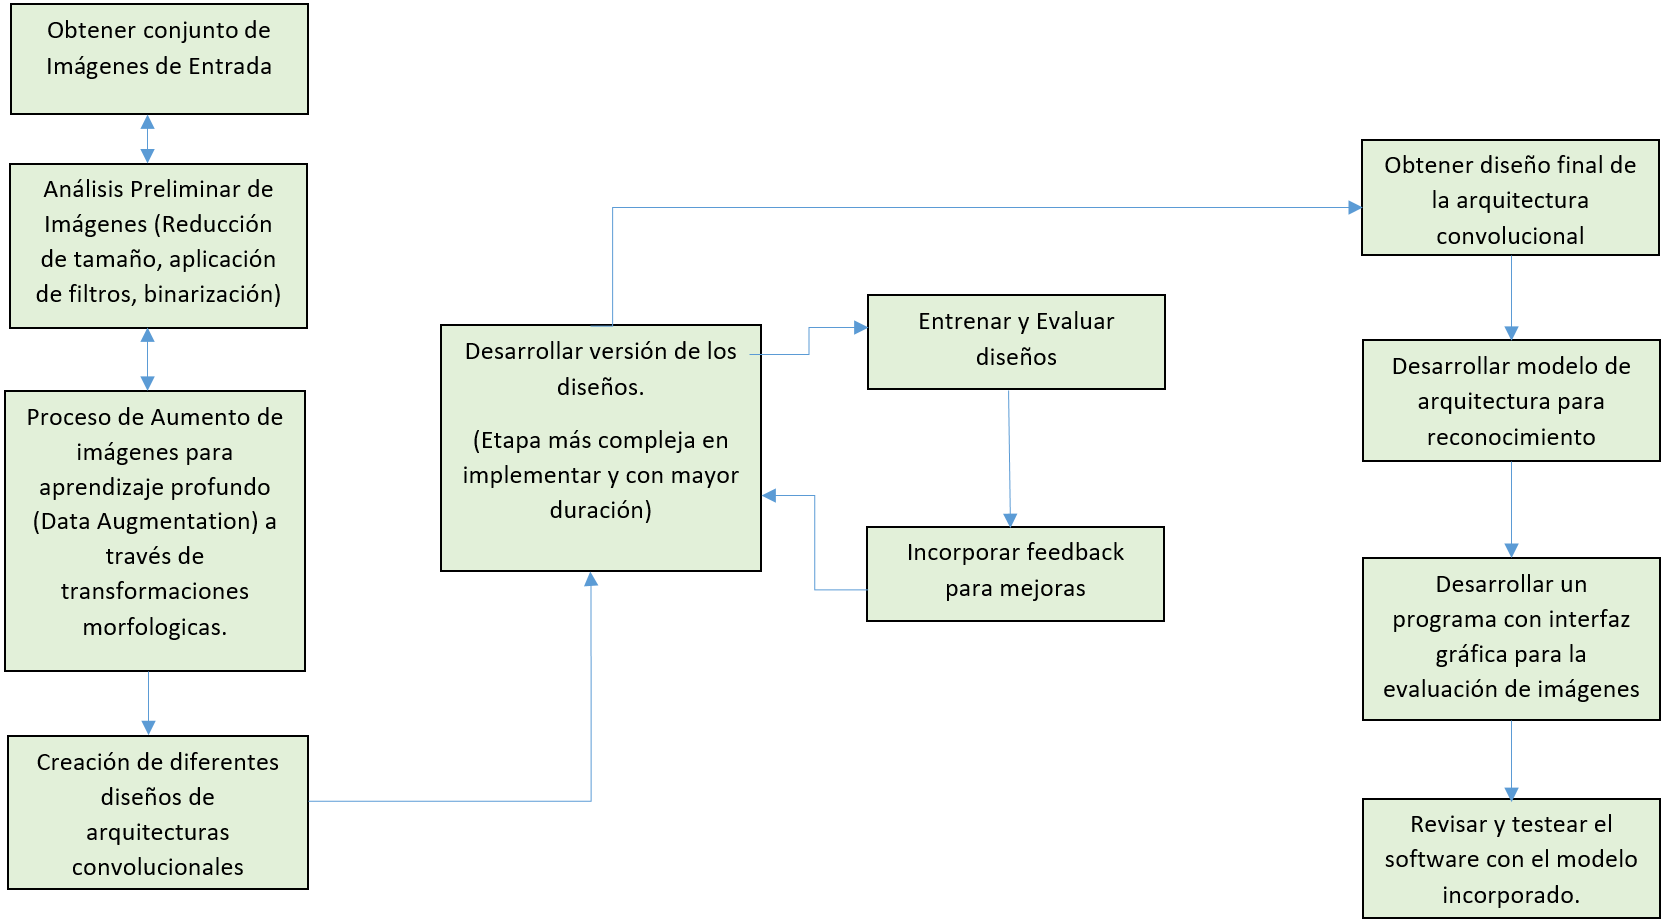
\includegraphics[width=0.9\textwidth]{images/intro/disenho}
			\end{center}
	
	\end{figure}
		

}



\frame{
\begin{block}
{\Large{Proceso de Desarrollo del Modelo}}
\end{block}
		
 	\begin{figure}[H]
	\begin{center}
	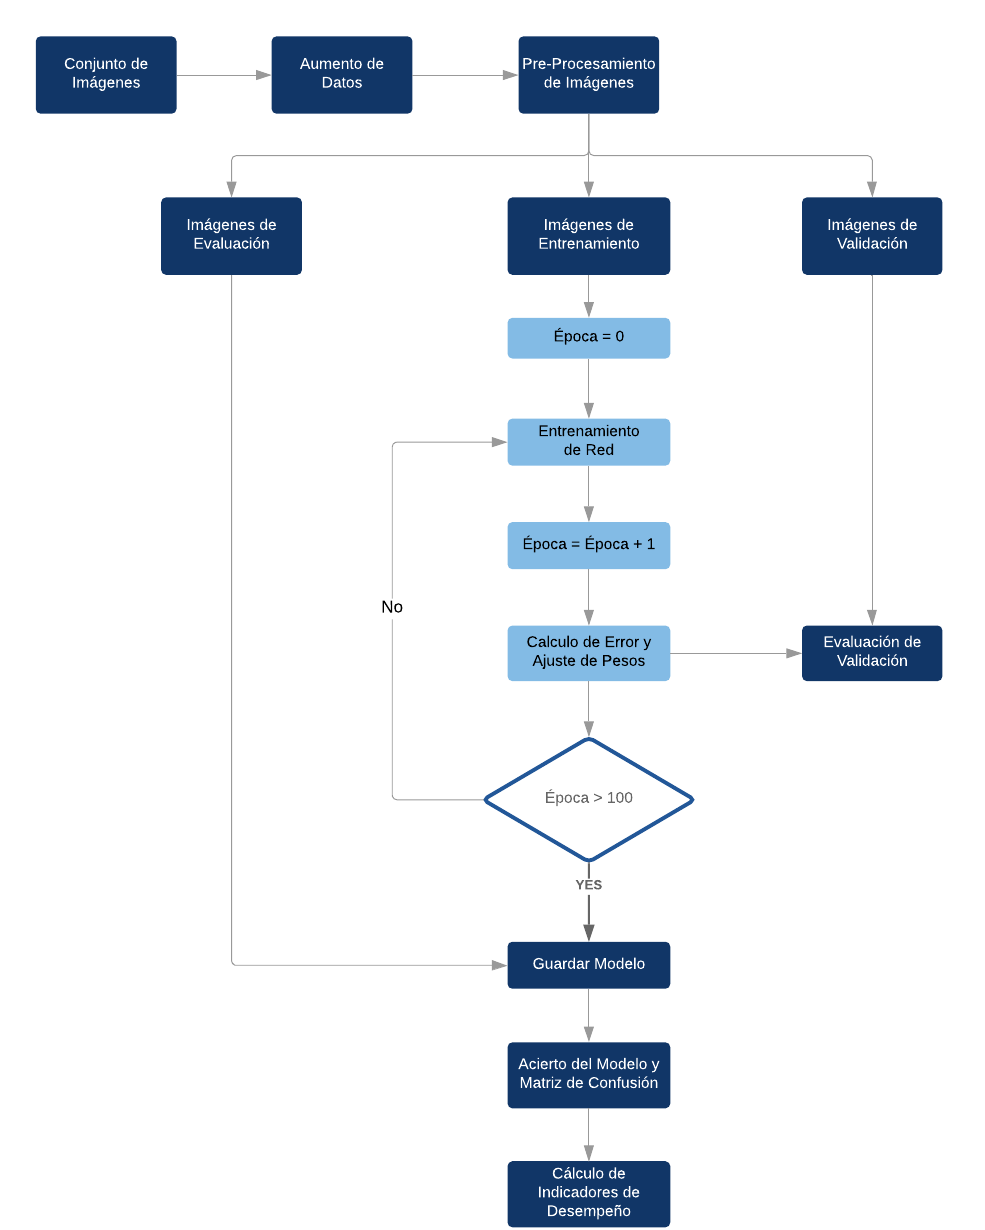
\includegraphics[width=1\textwidth, height=0.85\textheight,keepaspectratio]{images/summaryflowchart}
	\end{center}
	\vspace{1.5em}
	\begin{center}
	\caption{\small{Diagrama de flujo para el desarrollo de la Investigación}}
	\vskip -0.25cm
	{\small{Fuente: Elaboración propia}}
	\end{center}
\end{figure}
}



\frame{
\begin{block}
{\Large{Datos para el entrenamiento}}
\end{block}
%\vskip 0.5cm
	\begin{itemize}
	\item<1-> Señales de Tránsito de Alemania
	\begin{figure}[H]
				
				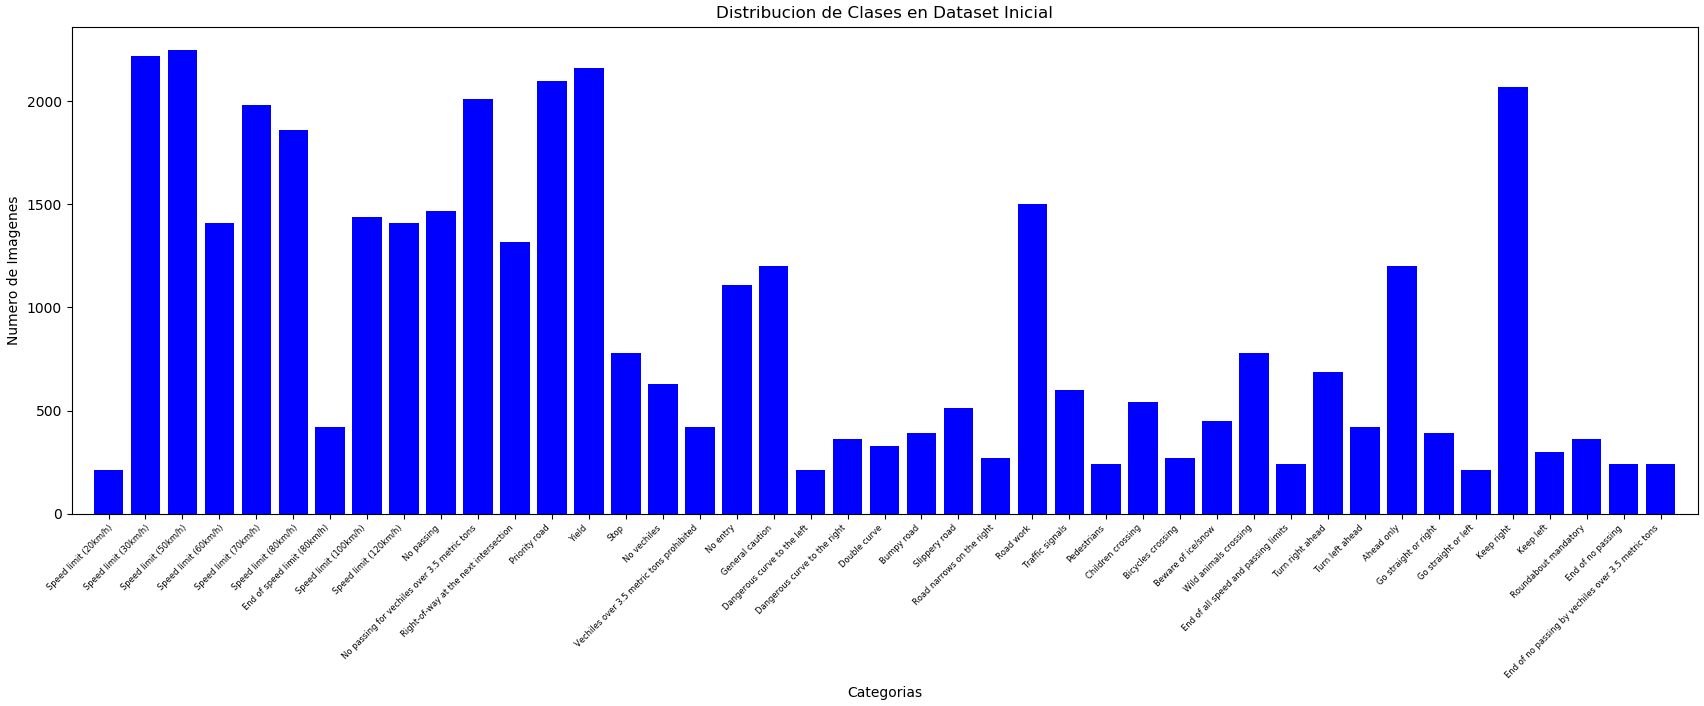
\includegraphics[width=0.9\textwidth,height=0.9\textheight,keepaspectratio]{images/desarrollo/histograms/initial39209}
				
				\begin{center}
				{\tiny{Distribución de ejemplos por señal para el entrenamiento(Total 39209)}}
			{\tiny {Fuente: Elaboración propia}}
				\end{center}
			\end{figure}
		
	\end{itemize}
}



\frame{
\begin{block}
{\Large{Datos para el entrenamiento}}
\end{block}
%\vskip 0.5cm
	\begin{itemize}

	\item<1->Señales de Tránsito de Perú
		\begin{figure}[H]
				\begin{center}
				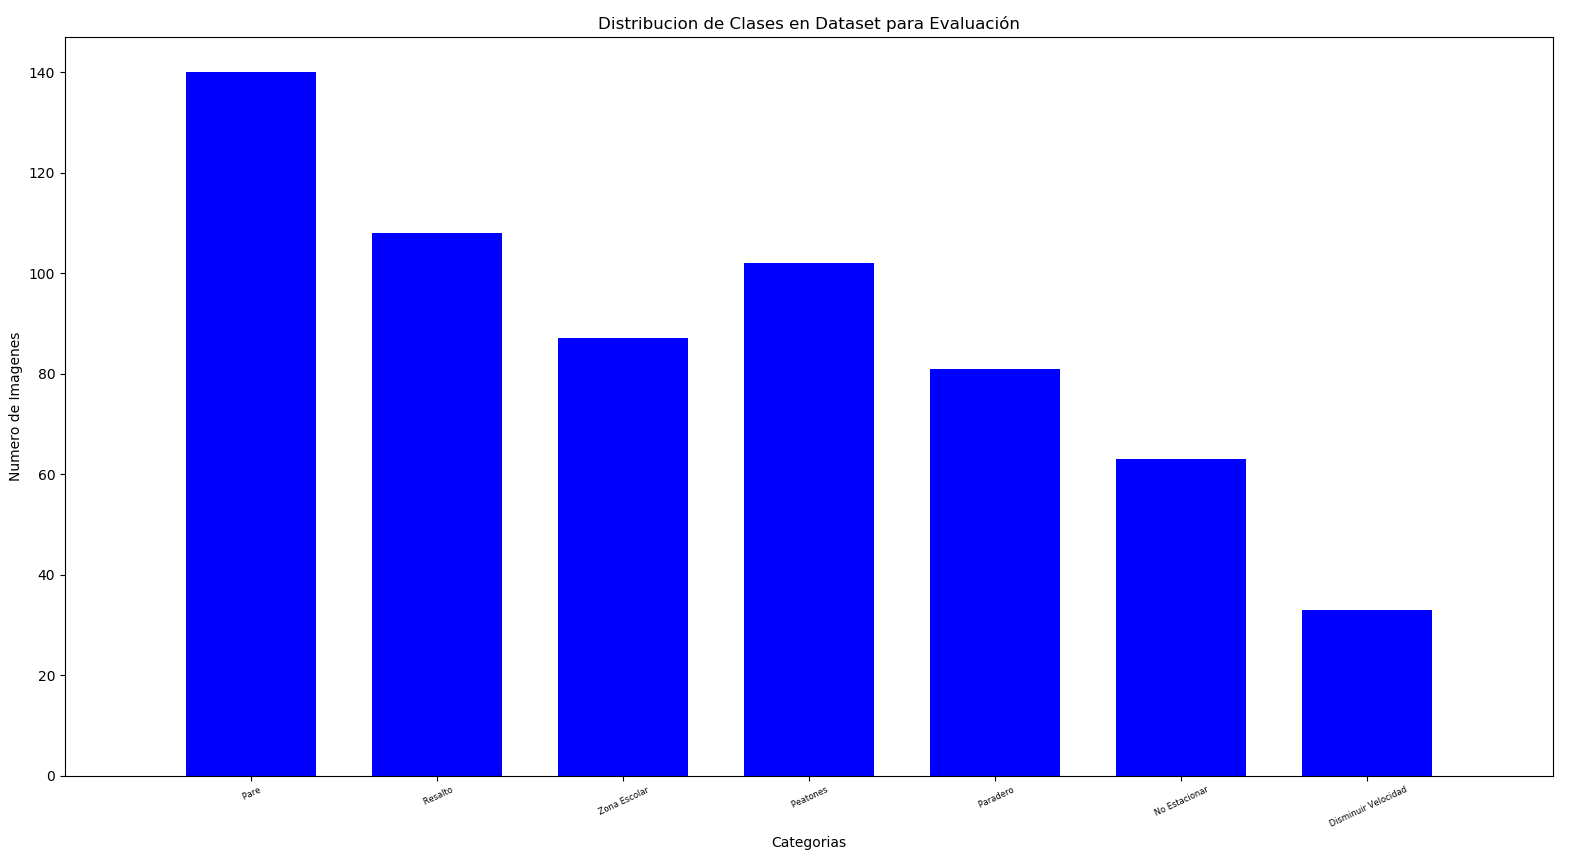
\includegraphics[width=0.9\textwidth,height=0.9\textheight,keepaspectratio]{images/desarrollo/histograms/inicioTrain614}
				\end{center}
				\begin{center}
				{\tiny{Distribución de ejemplos por señal para el entrenamiento(Total 614)}}
			{\tiny {Fuente: Elaboración propia}}
				\end{center}
			\end{figure}
	\end{itemize}
}




\frame{
\begin{block}
{\Large{Datos para la Evaluación}}
\end{block}
%\vskip 0.5cm
	\begin{itemize}
	\item<1-> Señales de Tránsito de Alemania (12630 imágenes)
	\begin{figure}[H]
				
				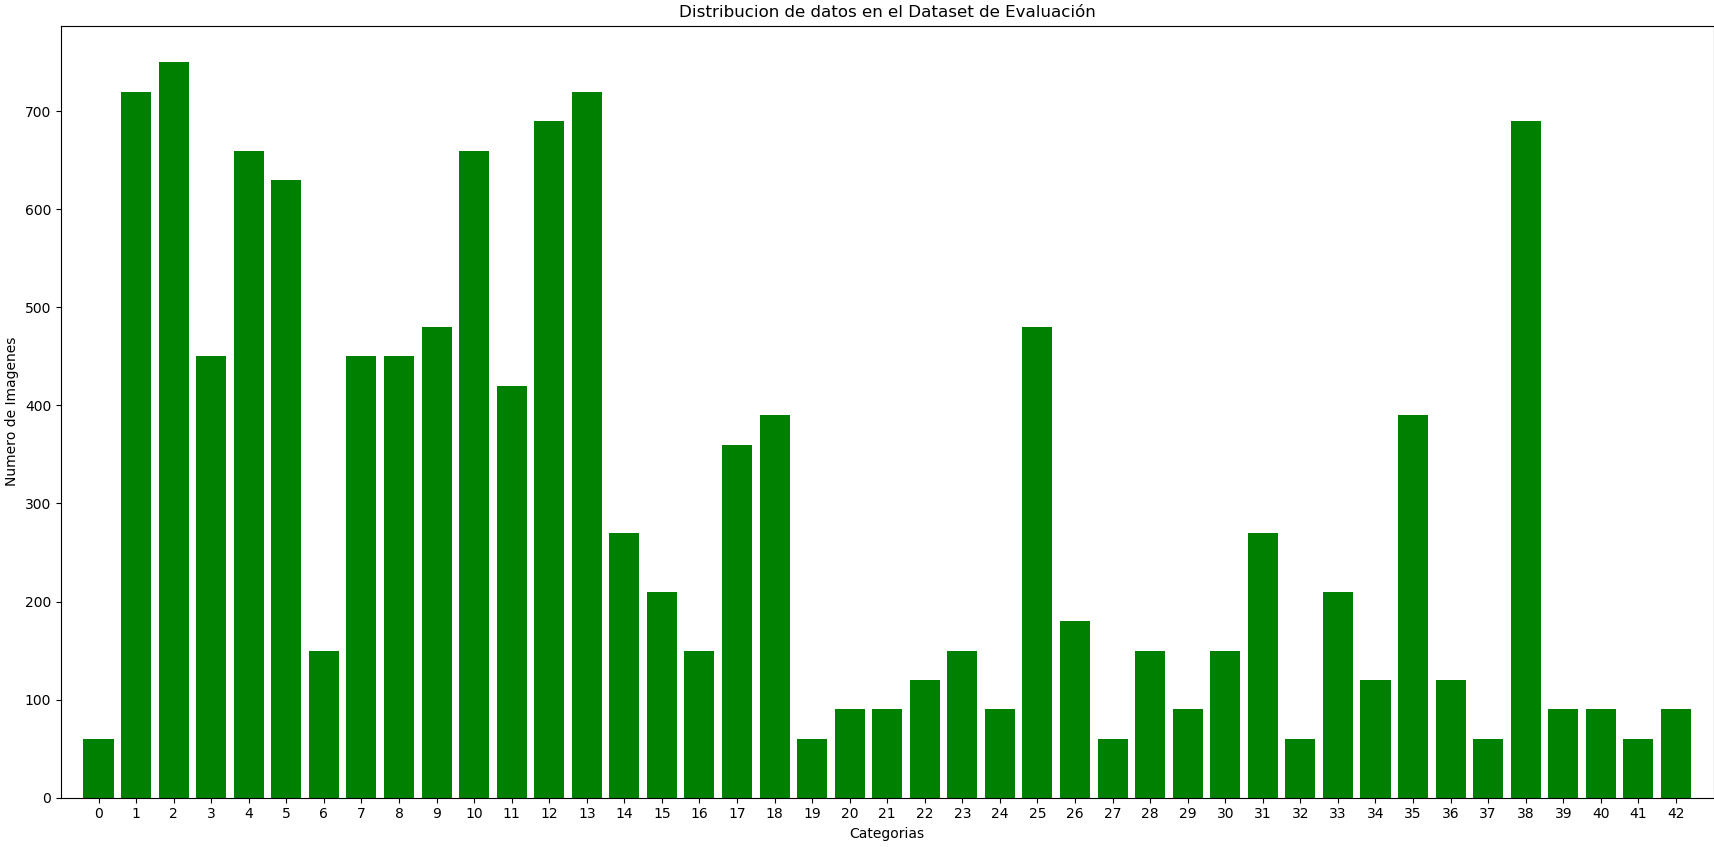
\includegraphics[width=0.9\textwidth,height=0.9\textheight,keepaspectratio]{images/desarrollo/histograms/initialTest12630}
				
				\begin{center}
				{\tiny{Distribución de ejemplos por señal para la evaluación - Alemania}}
				{\tiny {Fuente: Elaboración propia}}
				\end{center}
			\end{figure}
		
	\end{itemize}
}



\frame{
\begin{block}
{\Large{Datos para la Evaluación}}
\end{block}
%\vskip 0.5cm
	\begin{itemize}

	\item<1->Señales de Tránsito de Perú (4698 imágenes)
		\begin{figure}[H]
				\begin{center}
				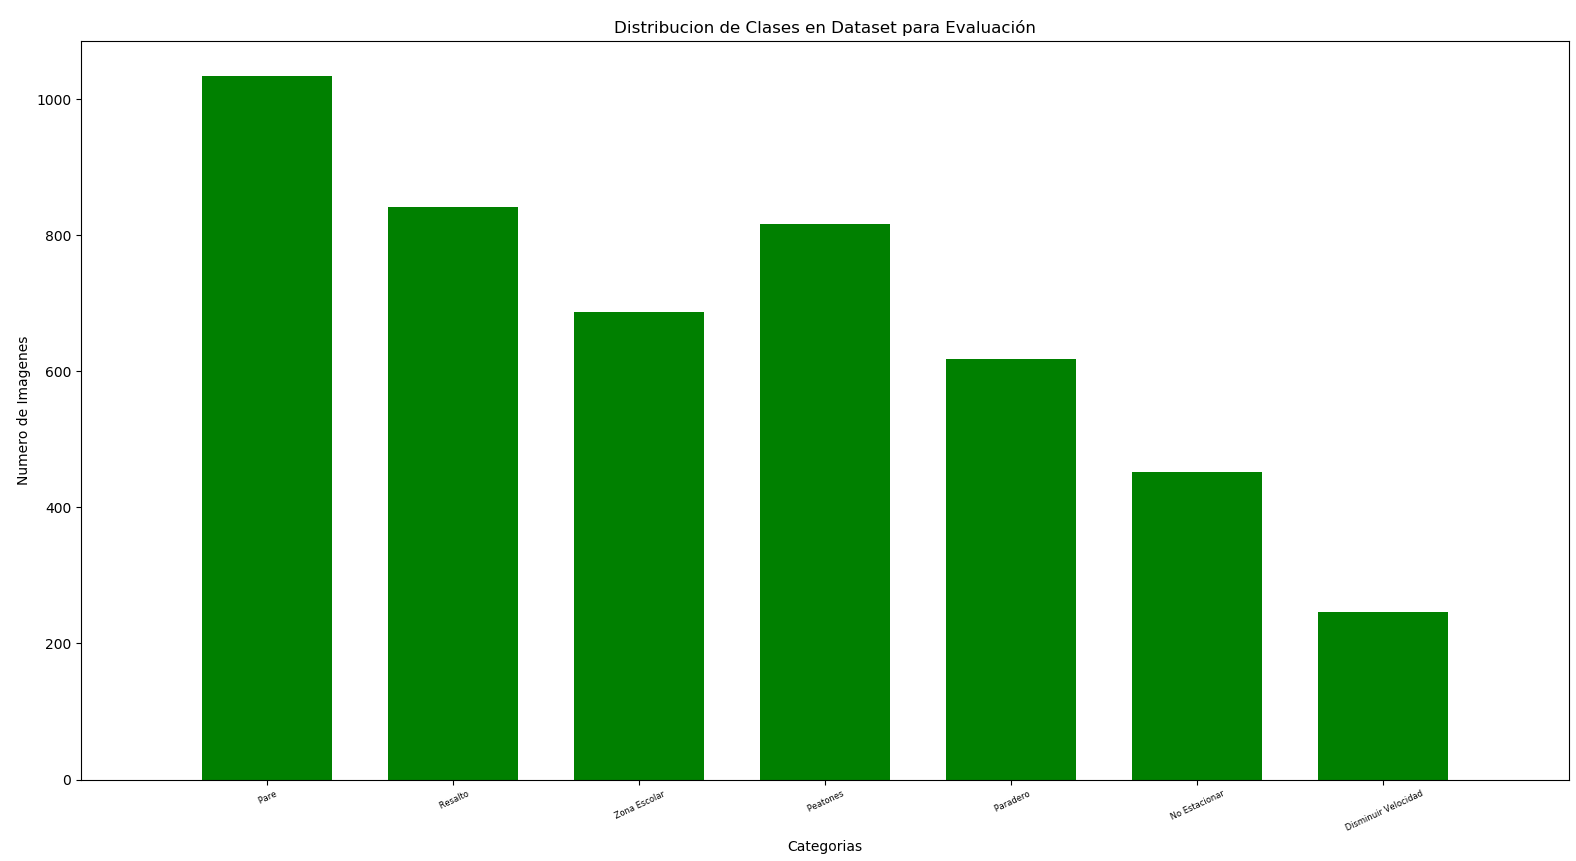
\includegraphics[width=0.9\textwidth,height=0.9\textheight,keepaspectratio]{images/desarrollo/histograms/PeruinitialTest4698}
				\end{center}
				\begin{center}
				{\tiny{Distribución de ejemplos por señal para la evaluación - Perú}}
				{\tiny {Fuente: Elaboración propia}}
				\end{center}
			\end{figure}
	\end{itemize}
}


%--------------------------------------Data Augmentation----------

\frame{
\begin{block}
{\Large{Proceso de Aumento de Datos(Data Augmentation)}}
\end{block}
	

	 \begin{enumerate}%\addtocounter{enumi}{2}
	\item Flipping
	\begin{multicols}{2}
				
				\underline{Flipping horizontal:}
				\begin{figure}[H]
					\begin{center}
					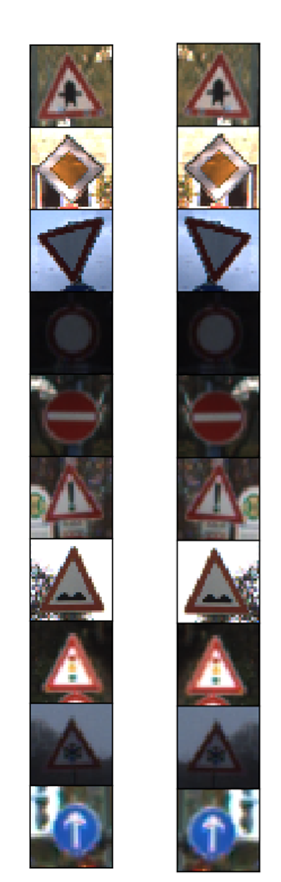
\includegraphics[width=0.7\textwidth,height=0.65\textheight,keepaspectratio]{images/desarrollo/Augment/flippedHorizontally}
					
					%\begin{center}\tiny{Imágenes volteadas horizontalmente}\end{center}
					%{\tiny{Ejemplo de Flipping Horizontal}}
				{\tiny {Fuente: Elaboración propia}}\end{center}
				\end{figure}

			%second column
			
				\underline{Flipping Vertical:}
				\begin{figure}[H]
					\begin{center}
					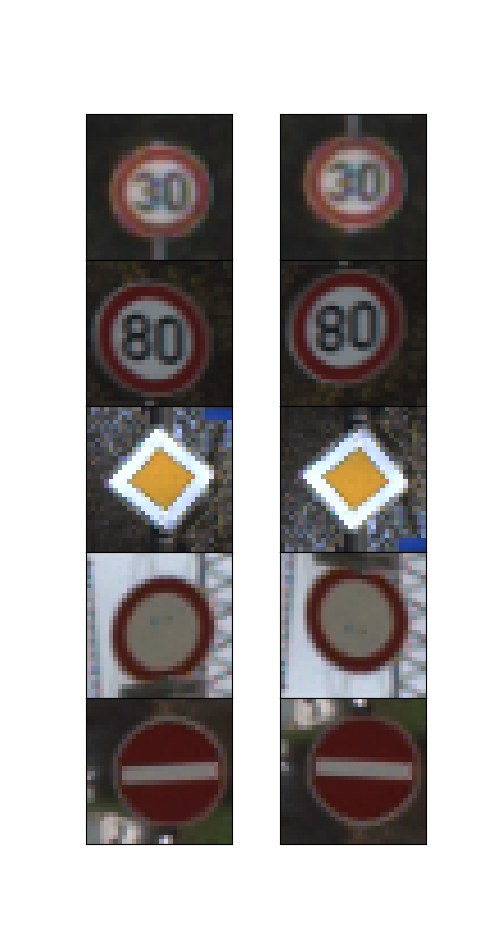
\includegraphics[width=0.7\textwidth,height=0.65\textheight,keepaspectratio]{images/desarrollo/Augment/flippableVertically}
					\vskip -0.5cm
					%\begin{center}\tiny{Imágenes volteadas verticalmente}\end{center}
				%{\tiny{Ejemplo de Flipping Vertical}}
				{\tiny {Fuente: Elaboración propia}}
				\end{center}
				\end{figure}

			\end{multicols}
	\end{enumerate}
}

\frame{
\begin{block}
{\Large{Proceso de Aumento de Datos(Data Augmentation)}}
\end{block}


	\underline{Flipping Horizontal y Vertical:}
			\begin{figure}[H]
				\begin{center}
				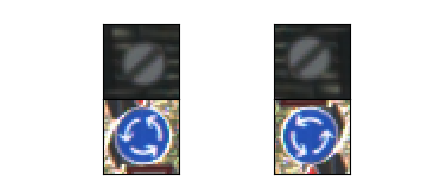
\includegraphics[width=0.7\textwidth,height=0.65\textheight,keepaspectratio ]{images/desarrollo/Augment/flippable_both}
				\end{center}
				
				%\tiny{Imágenes que volteadas horizontal o verticalmente, cambian su categoría}
				
			
			\end{figure}

}

\frame{
\begin{block}
{\Large{Proceso de Aumento de Datos(Data Augmentation)}}
\end{block}
	

	Incluso, hay signos que luego de voltearse, deben clasificarse como un signo de alguna otra clase. Esto sigue siendo útil, ya que podemos utilizar los datos de estas clases para ampliar sus contrapartes.
			\begin{figure}[H]
				\begin{center}
				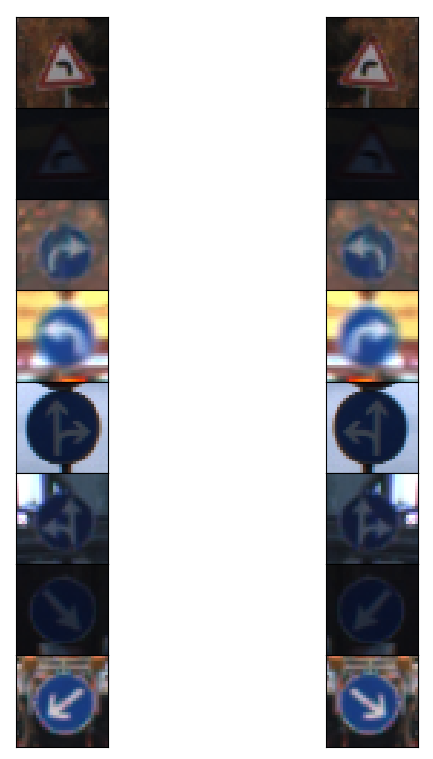
\includegraphics[width=0.7\textwidth,height=0.65\textheight,keepaspectratio ]{images/desarrollo/Augment/cross_flippable}
				\end{center}
				
				%\tiny{Imágenes que volteadas horizontal o verticalmente, cambian su categoría}
				
			
			\end{figure}

}



\frame{
\begin{block}
{\Large{Proceso de Aumento de Datos(Data Augmentation)}}
\end{block}
	

	Finalmente obtenemos una nueva distribución de datos luego de haber aplicado flipping a ciertas imagenes. Esta distribución consta de 63538 imágenes.
			\begin{figure}[H]
				\begin{center}
				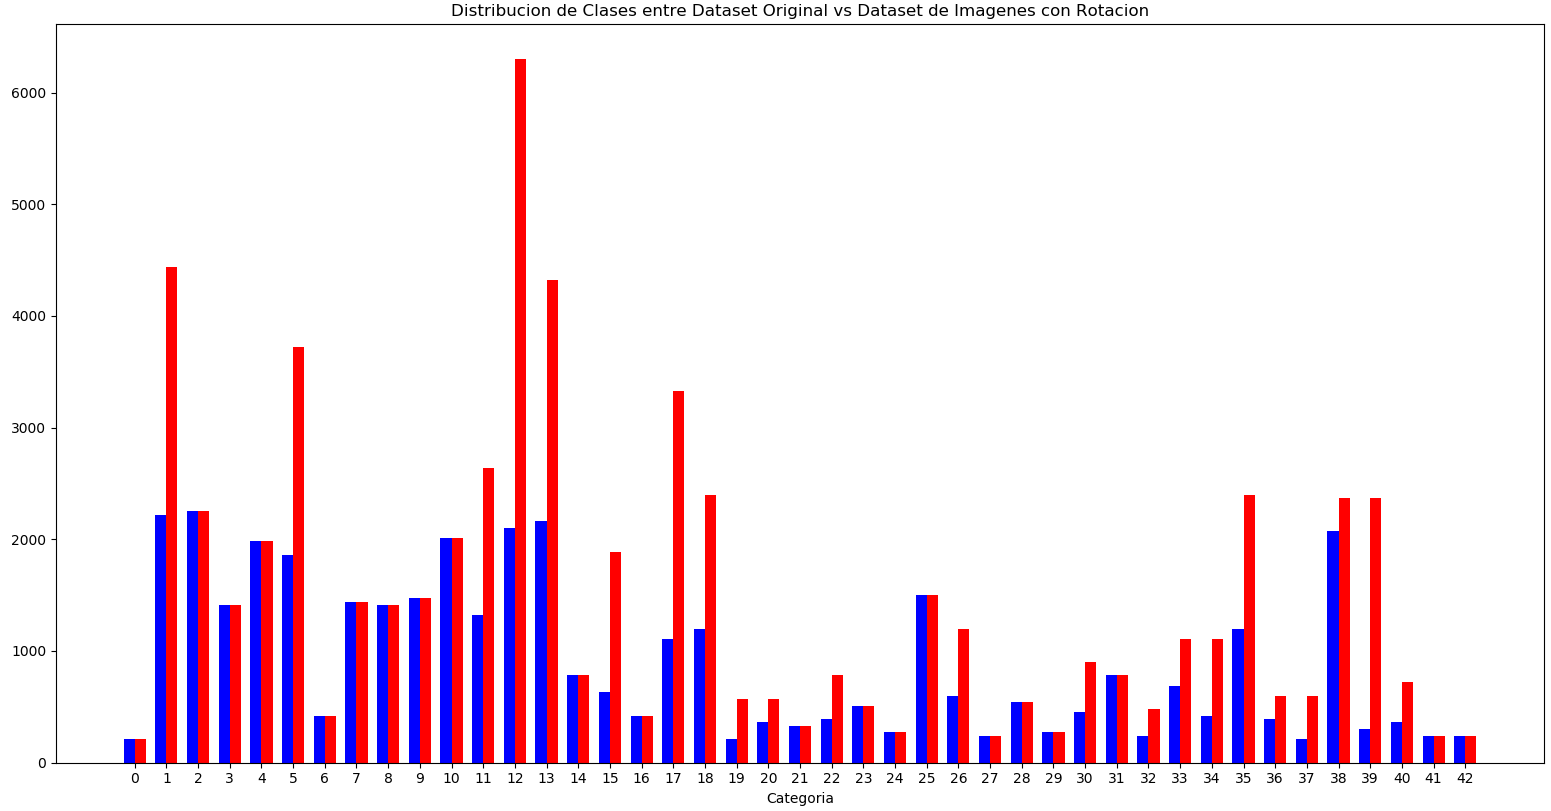
\includegraphics[width=0.8\textwidth,height=0.8\textheight,keepaspectratio]{images/desarrollo/histograms/train_flipped63538}
				\end{center}
				
				\vspace{-0.5em}
				\begin{center}
				{\tiny{Distribución de categoría, luego de aplicar el Flip(en sus distintos tipos)- Señales de Alemania}}\\
				{\tiny {Fuente: Elaboración propia}}
				\end{center}
			\end{figure}
}


\frame{
\begin{block}
{\Large{Proceso de Aumento de Datos(Data Augmentation)}}
\end{block}
	


	 \begin{enumerate}\addtocounter{enumi}{1}
	 	\item Projection(Proyección)
			\begin{figure}[H]
				\begin{center}
				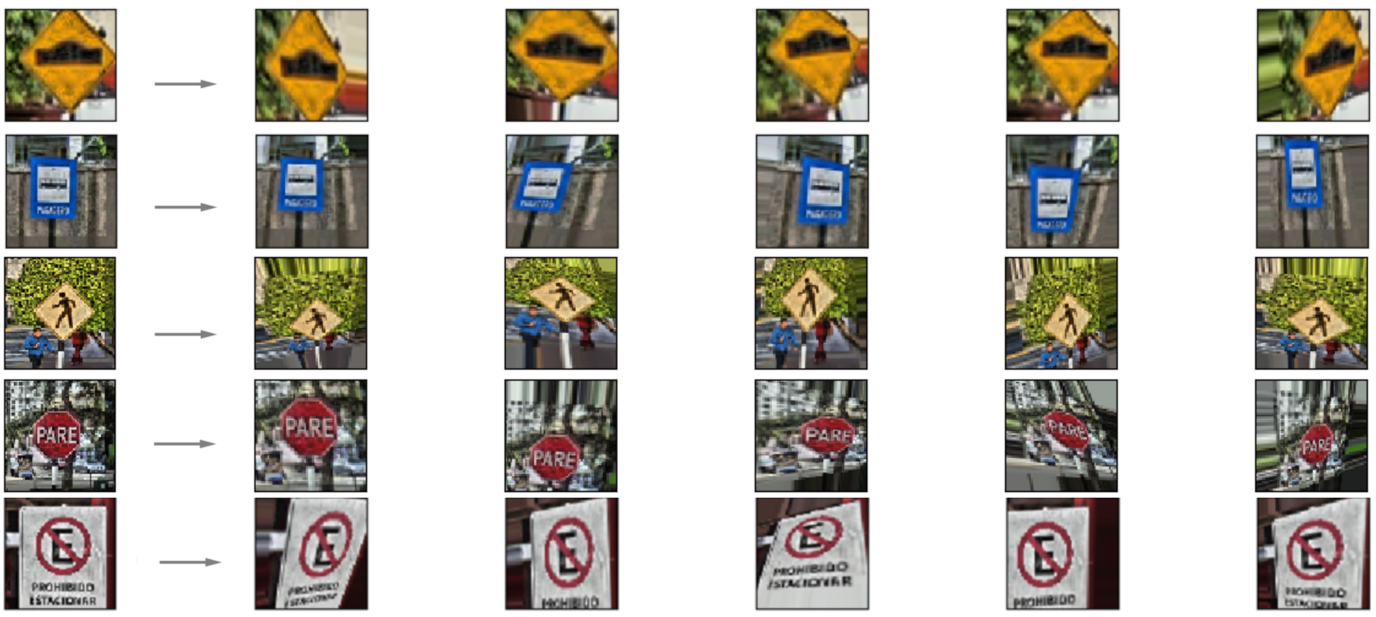
\includegraphics[width=0.8\textwidth,height=0.8\textheight,keepaspectratio]{images/desarrollo/Augment/projection_transform3}
				\end{center}
				{\tiny{Ejemplo de cinco proyecciones por cada imagen - Dataset Perú}}\\
				{\tiny {Fuente: Elaboración propia}}
					
			\end{figure}
		\end{enumerate}
}






\frame{
\begin{block}
{\Large{Proceso de Aumento de Datos(Data Augmentation)}}
\end{block}
	


	 \begin{enumerate}\addtocounter{enumi}{2}
	 	\item Rotation(Rotación)
			\begin{figure}[H]
				\begin{center}
				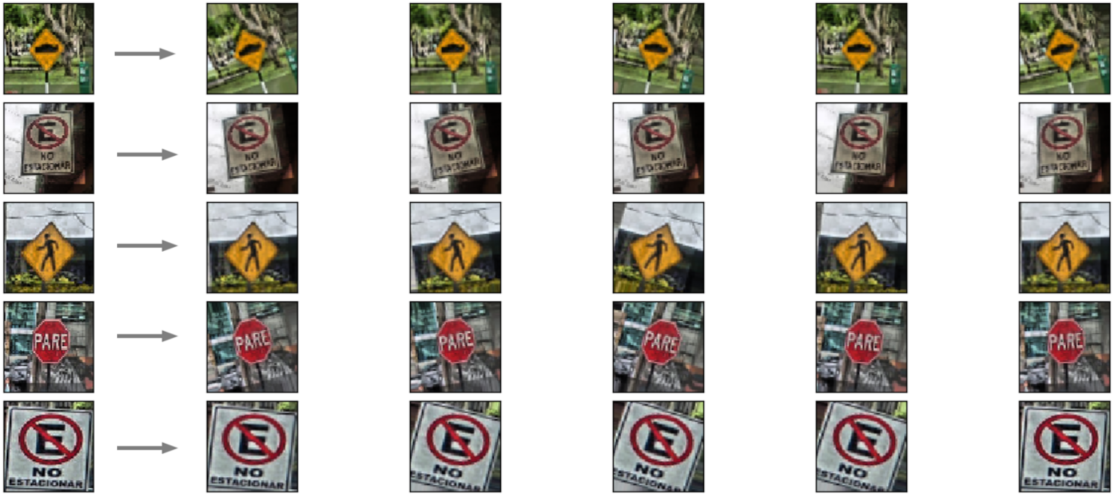
\includegraphics[width=0.8\textwidth,height=0.8\textheight,keepaspectratio]{images/desarrollo/Augment/fixedrotation2}
				\end{center}
				{\tiny{Ejemplo de cinco rotaciones por cada imagen - Dataset Perú}}\\
				{\tiny {Fuente: Elaboración propia}}

			\end{figure}
		\end{enumerate}
}



\frame{
\begin{block}
{\Large{Proceso de Aumento de Datos(Data Augmentation)}}
\end{block}
	


	 \begin{enumerate}\addtocounter{enumi}{3}
	 	\item Zoom
			\begin{figure}[H]
				\begin{center}
				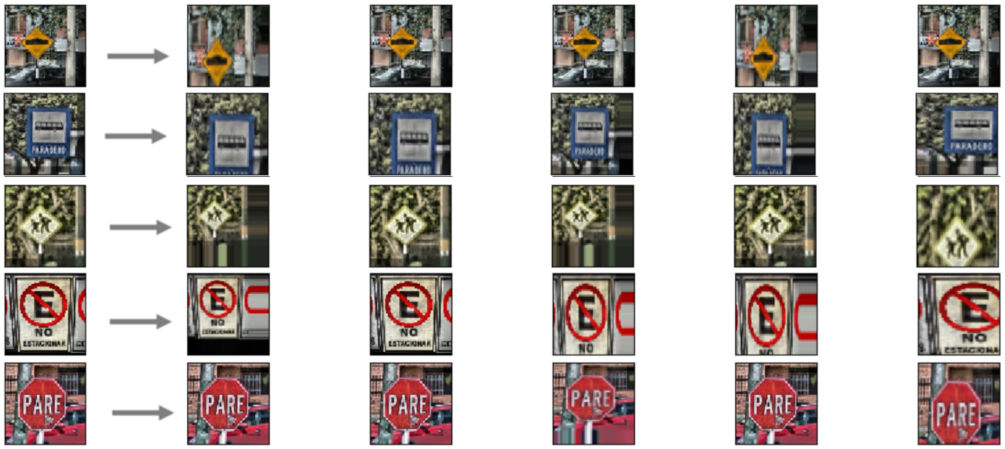
\includegraphics[width=0.8\textwidth,height=0.8\textheight,keepaspectratio]{images/desarrollo/Augment/zoom_inv2}
				\end{center}
				
				{\tiny{Ejemplo de cinco aplicaciones de zoom(in/out) por cada imagen - Dataset Perú}}\\
				{\tiny {Fuente: Elaboración propia}}

			\end{figure}
		\end{enumerate}
}

\frame{
\begin{block}
{\Large{Proceso de Aumento de Datos(Data Augmentation)}}
\end{block}
	


	 \begin{enumerate}\addtocounter{enumi}{4}
	 	\item Equalizacion del histograma
			\begin{figure}[H]
				\begin{center}
				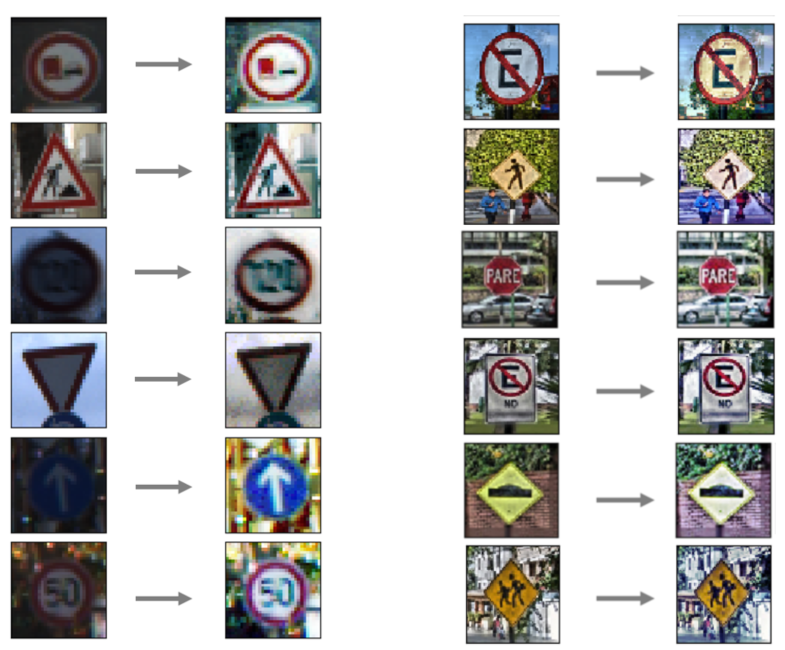
\includegraphics[width=0.8\textwidth,height=0.65\textheight,keepaspectratio]{images/desarrollo/Augment/equalize_hist2_wo_Norm_woRepetition2}
				\end{center}
				{\tiny{Distribución eficaz de los valores de intensidad más frecuentes}}\\
				{\tiny {Fuente: Elaboración propia}}
			\end{figure}
		\end{enumerate}
}

%------------------------------------------------------------------



\frame{
\begin{block}
{\Large{Dataset final }}
\end{block}
%\vskip 0.5cm
	\begin{itemize}
	\item<1-> Señales de Tránsito de Alemania (270900 imágenes)
	\begin{figure}[H]
				
				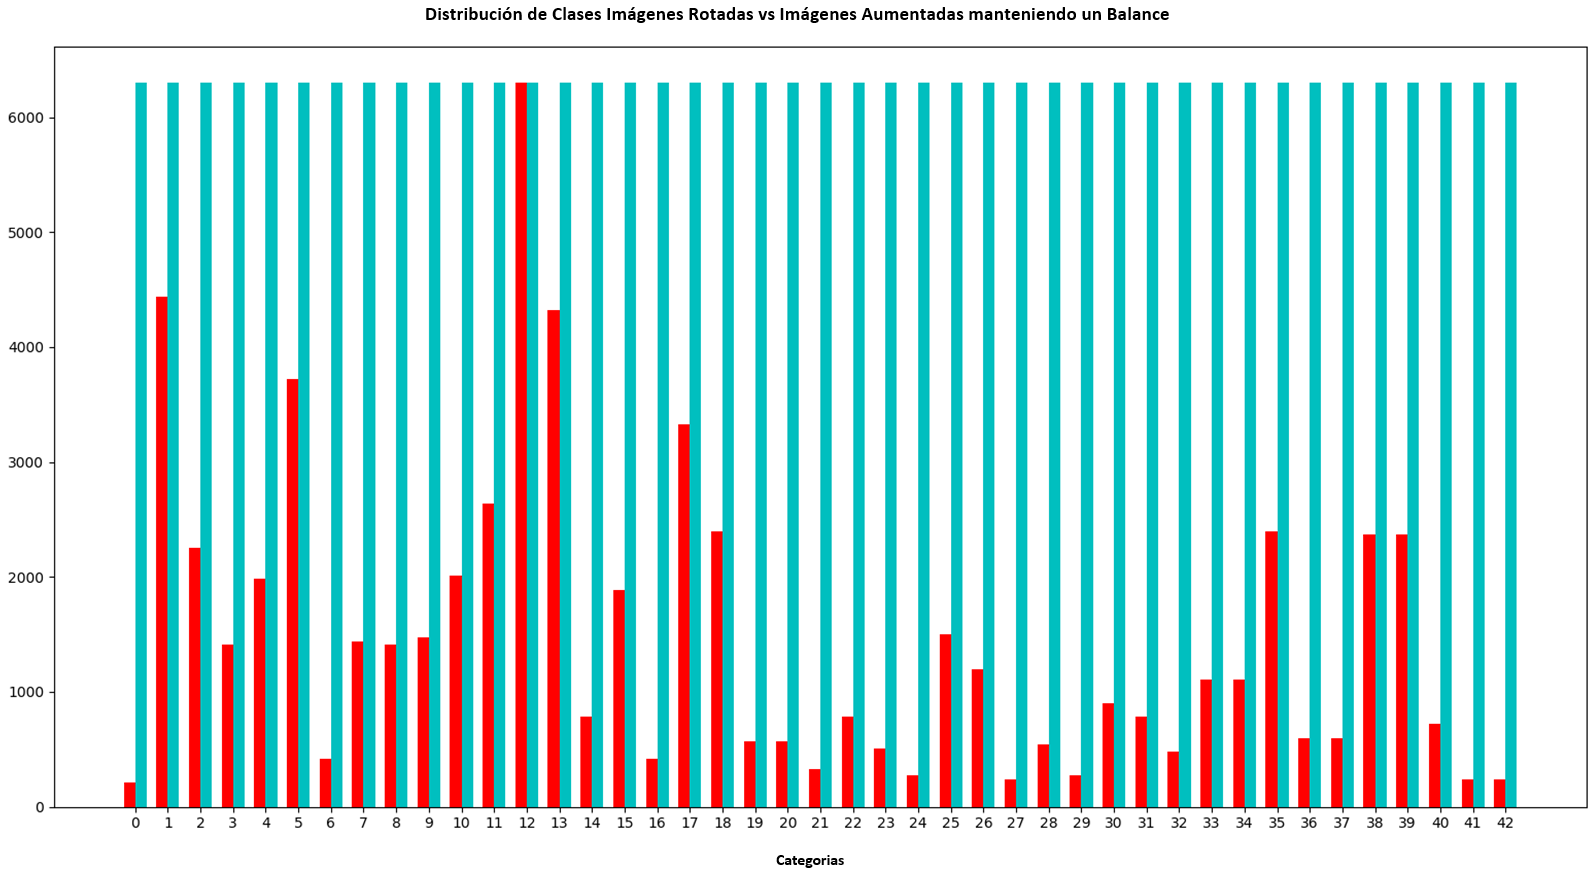
\includegraphics[width=0.9\textwidth,height=0.9\textheight,keepaspectratio]{images/desarrollo/histograms/train_extended_balanced270900}
				{\tiny {Fuente: Elaboración propia}}
			\end{figure}
		
	\end{itemize}
}

\frame{
\begin{block}
{\Large{Dataset final }}
\end{block}
%\vskip 0.5cm
	\begin{itemize}

	\item<1->Señales de Tránsito de Perú (31314 imágenes)
		\begin{figure}[H]
				
				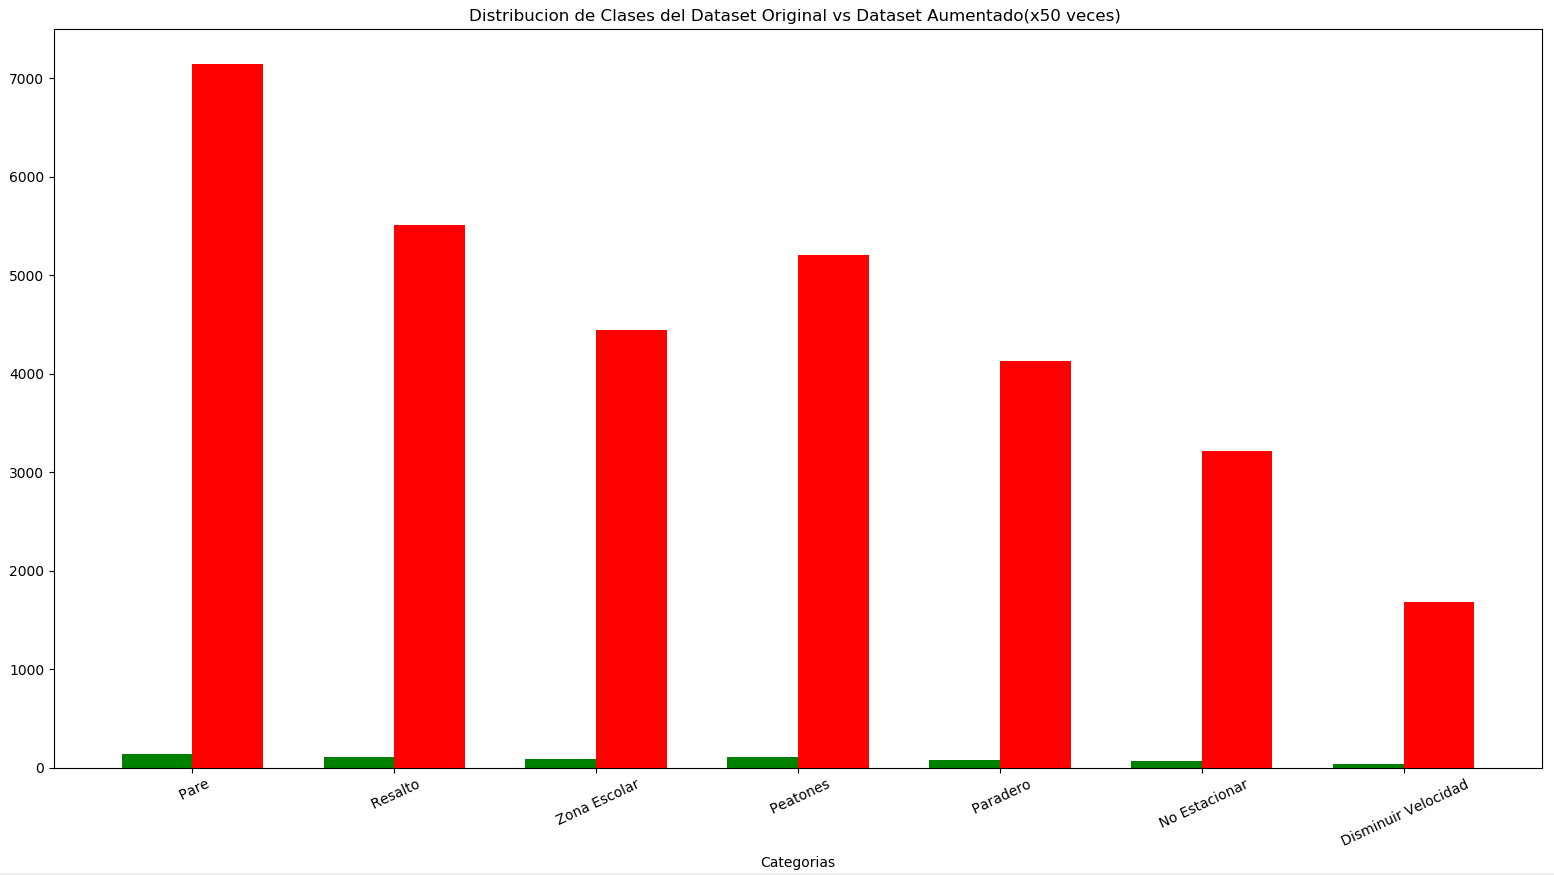
\includegraphics[width=0.9\textwidth,height=0.9\textheight,keepaspectratio]{images/desarrollo/histograms/train_extended_per_51_31314}
				{\tiny {Fuente: Elaboración propia}}
				
			\end{figure}
	\end{itemize}
}


\frame{
\begin{block}
{\Large{Dataset final }}
\end{block}
%\vskip 0.5cm
	\begin{table}[H]
	\begin{center}
				\caption{\small{Distribución Entrenamiento y Validación Dataset Balanceado - Señales de Tránsito de Alemania}}
				\begin{center}
				\begin{tabular}{|>{\scriptsize}c|>{\scriptsize}c|}
				\hline
				{\ul \textbf{CONJUNTO DE DATOS}}           & {\ul \textbf{CANTIDAD IMÁGENES}}                \\ \hline
				\textbf{Entrenamiento}                    & \text{203175}                       \\ \hline
				\textbf{Validación}                       & \text{67725}                    \\ \hline
				\textbf{Evaluación}                       & \text{12630}                    \\ \hline
				\end{tabular}
				\end{center}
				\begin{center}
				%\vskip 0.3cm
				{\tiny{Fuente: Elaboración propia.}}
				\end{center}
				\end{center}
			\end{table}

	\begin{table}[H]
	\begin{center}
		\caption{\small{Distribución Entrenamiento y Validación Dataset no Balanceado - Señales de Tránsito de Perú}}
		\begin{center}
		\begin{tabular}{|>{\scriptsize}c|>{\scriptsize}c|}
		\hline
		{\ul \textbf{CONJUNTO DE DATOS}}           & {\ul \textbf{CANTIDAD IMÁGENES}}     \\ \hline
		\textbf{Entrenamiento}                    & \text{23485 }                   \\ \hline
		\textbf{Validación}                       & \text{3131 }                    \\ \hline
		\textbf{Evaluación}                       & \text{4698 }                    \\ \hline
		\end{tabular}
		\end{center}
		\begin{center}
		%\vskip 0.3cm
		{\tiny{Fuente: Elaboración propia.}}
		\end{center}
		\end{center}
	\end{table}
}


\frame{
\begin{block}
{\Large{Pre-procesamiento de Imágenes(Normalization) }}
\end{block}
%\vskip 0.5cm
	\begin{itemize}

	\item<1->La técnica utilizada CLAHE es un algoritmo para la mejora del contraste local, que utiliza histogramas calculados sobre diferentes regiones en una imagen.
	\vskip 0.2cm
	\item<2->Difiere de la ecualización de histograma ordinaria en el sentido de que el método adaptativo computa varios histogramas, cada uno correspondiente a una sección distinta de la imagen, y los utiliza para redistribuir los valores de luminosidad de la imagen.
	\vskip 0.2cm
	\item<3->Mejora el nivel de visibilidad de una imagen o video con niebla ya que permite mejorar los detalles locales incluso en regiones que son más oscuras o más claras que la mayoría de regiones de la imagen. \citep{CLAHE}
		\begin{figure}[H]
				\begin{center}
				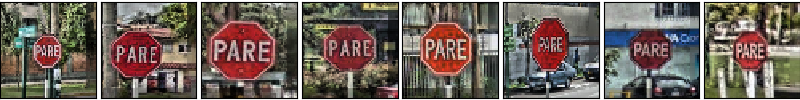
\includegraphics[width=0.9\textwidth,height=0.9\textheight,keepaspectratio]{images/desarrollo/Normalization_Processing/norm_test3}
				\end{center}
			\end{figure}
	\end{itemize}
}


\frame{
\begin{block}
{\Large{Pre-procesamiento de Imágenes(Normalization) }}
\end{block}
%\vskip 0.5cm
	\begin{itemize}

	\item<1->Pierre Sermanet y Yann LeCun mencionaron en su artículo \citep{LeCun}, que el uso de canales de color no pareció mejorar mucho las cosas. Además, debido a diversas condiciones o problemas de iluminación, no es adecuado procesar directamente las imágenes que se capturan a través de la cámara o sensores de imágenes, es por ello que en esta investigación {\bf se usará un solo canal} en el modelo, es decir las imágenes estarán en escala de grises en lugar de tener 3 canales de colores.

		\begin{figure}[H]
				\begin{center}
				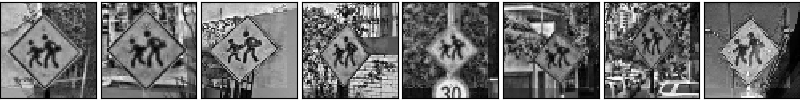
\includegraphics[width=0.9\textwidth,height=0.9\textheight,keepaspectratio]{images/desarrollo/Normalization_Processing/proc_test4}
				\end{center}
			\end{figure}
	\end{itemize}
}


\frame{
\begin{block}
{\Large{Arquitectura del Modelo }}
\end{block}
%\vskip 0.5cm
	\begin{itemize}

	\item<1->Los hiperparámetros engloban funciones, variables y constantes utilizadas durante la construcción de las diferentes arquitecturas; estas varían, sin embargo siguiendo conceptos teóricos, antecedentes (investigaciones previas) y sobretodo despues de algunas pruebas realizadas, los siguientes hiperparámetros fueron seleccionados de manera específica:

	\begin{table}[H]
		\begin{center}
			\caption{\small{Hiperparámetros del Modelo}}
			\vskip -0.2cm
			\begin{tabular}{|>{\tiny}c|>{\tiny}c|>{\tiny}c|>{\tiny}c|}
			\hline
			{\ul \textbf{HIPERPARÁMETROS}}  & {\ul \textbf{TIPO}}       & {\ul \textbf{HIPERPARÁMETROS}}        & {\ul \textbf{TIPO}}        \\ \hline
			{\textbf{Tasa de Aprendizaje - Alemania}}                     		& {\textit{0.0005 (5e-4)}}  				  &
			\textbf{Tasa de Aprendizaje - Perú}                                & \textit{0.0001 (1e-4)}                    \\ \hline
			\textbf{Alg. de Optimización}                               & \textit{Optimizador Adam}          &
			\textbf{Método de Validación}                               & \textit{Entropía Cruzada}          \\ \hline
			\textbf{Fun. Activ. Capas Convolucionales}        			& \textit{RELU y DropOut}                      &
			\textbf{Fun. Activ. Capas Totalmente Conectadas} 			& \textit{Func. Softmax}           \\ \hline
			\textbf{Método de Regularización}                           &\textit{L2 Lasso(lambda = 0.0001)} &
			\textbf{Épocas}                                             &\textit{100}		 				\\ \hline
			\end{tabular}
			
			\begin{center}
				\vskip 0.2cm
				{\tiny{Fuente: Elaboración propia.}}
				\end{center}
			\end{center}
		\end{table}

	\end{itemize}
}

\frame{
\begin{block}
{\Large{Modelos Propuestos }}
\end{block}
%\vskip 0.5cm
	\begin{enumerate}%\addtocounter{enumi}{4}

	\item MODELO A 
	\vskip 0.3cm
	\underline{Alemania}
	\begin{table}[H]
			\begin{center}
			\caption{\small{Diseño A (19'057952 neuronas) - Dataset de Imágenes de Alemania}}
			\setlength{\tabcolsep}{2pt}
			\begin{tabular}{|>{\tiny}c|>{\tiny}c>{\tiny}c>{\tiny}c>{\tiny}c>{\tiny}c|>{\tiny}c|}
			\hline
			{\color[HTML]{000000} \textbf{Capa}} & {\color[HTML]{000000} \textbf{Entrada}} & {\color[HTML]{000000} \textbf{Tipo}} & {\color[HTML]{000000} \textbf{\begin{tabular}[c]{@{}c@{}}Número de\\ (kernels/filtros)\end{tabular}}} & {\color[HTML]{000000} \textbf{Padding}} & {\textbf{Salida}} & {\textbf{Func.Esc.Múltiple}}\\ \hline

				 & 1 de 32 x 32  & Conv(DropOut : 0.8) & 32 de 3 x 3 neuronas & Activo & 32 de 32 x 32 & --\\ 
				\multirow{-2}{*}{1} &  32 de 32 x 32  &  Max Pool &  32 de 2 x 2 &  Inactivo & 32 de 16 x 16  & {\cellcolor[HTML]{DAE8FC}(MaxPool = 2) 32 de 8x8}\\ \hline
				 & 32 de 16 x 16  & Conv(DropOut : 0.7) & 64 de 5 x 5 neuronas & Activo & 64 de 16 x 16 & --\\ 
				\multirow{-2}{*}{2} &  64 de 16 x 16  &  Max Pool &  64 de 2 x 2 &  Inactivo & 64 de 8 x 8  & {\cellcolor[HTML]{DAE8FC}(MaxPool = 1) 64 de 8x8}\\ \hline
				3 &  {\cellcolor[HTML]{DAE8FC}6144 neuronas} &  F.C.(DropOut : 0.5) &  3072 neuronas &  -- & 43  & --\\ \hline

			\end{tabular}
			\end{center}
			\begin{center}
			\vskip 0.2cm
			{\small{Fuent0e: Elaboración propia.}}
			\end{center}
			\end{table}
	\end{enumerate}
}



\frame{
\begin{block}
{\Large{Modelos Propuestos }}
\end{block}
%\vskip 0.5cm
	\begin{enumerate}%\addtocounter{enumi}{4}

	\item MODELO A 
\vskip 0.3cm
	\underline{Perú}
		\begin{table}[H]
			\begin{center}
			\caption{\small{Diseño A (66'428192 neuronas) - Dataset de Imágenes de Perú}}
			\setlength{\tabcolsep}{2pt}
			\begin{tabular}{|>{\tiny}c|>{\tiny}c>{\tiny}c>{\tiny}c>{\tiny}c>{\tiny}c|>{\tiny}c|}
			\hline
			{\color[HTML]{000000} \textbf{Capa}} & {\color[HTML]{000000} \textbf{Entrada}} & {\color[HTML]{000000} \textbf{Tipo}} & {\color[HTML]{000000} \textbf{\begin{tabular}[c]{@{}c@{}}Número de\\ (kernels/filtros)\end{tabular}}} & {\color[HTML]{000000} \textbf{Padding}} & {\textbf{Salida}} & {\textbf{Func.Esc.Múltiple}}\\ \hline

				 & 1 de 60 x 60 & Conv(DropOut : 0.8) & 32 de 3 x 3 neuronas & Activo & 32 de 60 x 60  & --\\ 
				\multirow{-2}{*}{1} &  32 de 60 x 60  &  Max Pool &  32 de 2 x 2 &  Inactivo & 32 de 30 x 30  & {\cellcolor[HTML]{DAE8FC}(MaxPool = 2) 32 de 15x15}\\ \hline
				 & 32 de 30 x 30  & Conv(DropOut : 0.7) & 64 de 5 x 5 neuronas & Activo & 64 de 30 x 30  & --\\ 
				\multirow{-2}{*}{2} &  64 de 30 x 30  &  Max Pool &  64 de 2 x 2 &  Inactivo & 64 de 15 x 15  & {\cellcolor[HTML]{DAE8FC}(MaxPool = 1) 64 de 15x15}\\ \hline
				3 &  {\cellcolor[HTML]{DAE8FC}21600 neuronas} &  F.C.(DropOut : 0.5) &  7200 neuronas &  -- & 7  & --\\ \hline

			\end{tabular}
			\end{center}
			\begin{center}
			\vskip 0.2cm
			{\small{Fuente: Elaboración propia.}}
			\end{center}
		\end{table}
	\end{enumerate}
}










\frame{
\begin{block}
{\Large{Modelos Propuestos }}
\end{block}
%\vskip 0.5cm
	\begin{enumerate}\addtocounter{enumi}{1}

	\item MODELO B
\vskip 0.3cm
	\underline{Alemania}
		\begin{table}[H]
			\begin{center}
			\caption{\small{Diseño B (3'970336 neuronas) - Dataset de Imágenes de Alemania}}
			\setlength{\tabcolsep}{2pt}
			\begin{tabular}{|>{\tiny}c|>{\tiny}c>{\tiny}c>{\tiny}c>{\tiny}c>{\tiny}c|>{\tiny}c|}
			\hline
			{\color[HTML]{000000} \textbf{Capa}} & {\color[HTML]{000000} \textbf{Entrada}} & {\color[HTML]{000000} \textbf{Tipo}} & {\color[HTML]{000000} \textbf{\begin{tabular}[c]{@{}c@{}}Número de\\ (kernels/filtros)\end{tabular}}} & {\color[HTML]{000000} \textbf{Padding}} & {\textbf{Salida}} & {\textbf{Func.Esc.Múltiple}}\\ \hline

				 & 1 de 32 x 32  & Conv(DropOut : 0.8) & 32 de 3 x 3 neuronas& Activo & 32 de 32 x 32  & --\\ 
				\multirow{-2}{*}{1} &  32 de 32 x 32  &  Max Pool &  32 de 2 x 2 &  Inactivo & 32 de 16 x 16  & {\cellcolor[HTML]{DAE8FC}(MaxPool = 4) 32 de 4x4}\\ \hline
				 & 32 de 16 x 16  & Conv(DropOut : 0.7) & 64 de 5 x 5 neuronas& Activo & 64 de 16 x 16  & --\\ 
				\multirow{-2}{*}{2} &  64 de 16 x 16  &  Max Pool &  64 de 2 x 2 &  Inactivo & 64 de 8 x 8  & {\cellcolor[HTML]{DAE8FC}(MaxPool = 2) 64 de 4x4}\\ \hline			
				{\cellcolor[HTML]{ffb3b3}} & 64 de 8 x 8  & Conv(DropOut : 0.6) & 128 de 5 x 5 neuronas & Activo & 128 de 8 x 8  & --\\ 			
				{\cellcolor[HTML]{ffb3b3} \multirow{-2}{*}{3}} &  128 de 8 x 8  &  Max Pool &  128 de 2 x 2 &  Inactivo & 128 de 4 x 4  & {\cellcolor[HTML]{DAE8FC} (MaxPool = 1) 128 de 4x4 }\\ \hline
				4 &  {\cellcolor[HTML]{DAE8FC}3584 neuronas} &  F.C.(DropOut : 0.5) &  1024 neuronas &  -- & 43  & --\\ \hline
			\end{tabular}
			\end{center}
			\begin{center}
			\vskip 0.2cm
			{\small{Fuente: Elaboración propia.}}
			\end{center}
			\end{table}
	\end{enumerate}
}



\frame{
\begin{block}
{\Large{Modelos Propuestos }}
\end{block}
%\vskip 0.5cm
	\begin{enumerate}\addtocounter{enumi}{1}

	\item MODELO B
\vskip 0.3cm
	\underline{Perú}
		\begin{table}[H]
			\begin{center}
			\caption{\small{Diseño B (29'910388 neuronas) - Dataset de Imágenes de Perú}}
			\setlength{\tabcolsep}{2pt}
			\begin{tabular}{|>{\tiny}c|>{\tiny}c>{\tiny}c>{\tiny}c>{\tiny}c>{\tiny}c|>{\tiny}c|}
			\hline
			{\color[HTML]{000000} \textbf{Capa}} & {\color[HTML]{000000} \textbf{Entrada}} & {\color[HTML]{000000} \textbf{Tipo}} & {\color[HTML]{000000} \textbf{\begin{tabular}[c]{@{}c@{}}Número de\\ (kernels/filtros)\end{tabular}}} & {\color[HTML]{000000} \textbf{Padding}} & {\textbf{Salida}} & {\textbf{Func.Esc.Múltiple}}\\ \hline

				 & 1 de 60 x 60  & Conv(DropOut : 0.8) & 32 de 3 x 3 neuronas& Activo & 32 de 60 x 60  & --\\ 
				\multirow{-2}{*}{1} &  32 de 60 x 60  &  Max Pool &  32 de 2 x 2 &  Inactivo & 32 de 30 x 30  & {\cellcolor[HTML]{DAE8FC}(MaxPool = 4) 32 de 7x7}\\ \hline
				 & 32 de 30 x 30  & Conv(DropOut : 0.7) & 64 de 5 x 5 neuronas& Activo & 64 de 30 x 30  & --\\ 
				\multirow{-2}{*}{2} &  64 de 30 x 30  &  Max Pool &  64 de 2 x 2 &  Inactivo & 64 de 15 x 15  & {\cellcolor[HTML]{DAE8FC}(MaxPool = 2) 64 de 7x7}\\ \hline			
				{\cellcolor[HTML]{ffb3b3}} & 64 de 15 x 15  & Conv(DropOut : 0.6) & 128 de 5 x 5 neuronas & Activo & 128 de 15 x 15  & --\\ 			
				{\cellcolor[HTML]{ffb3b3} \multirow{-2}{*}{3}} &  128 de 15 x 15  &  Max Pool &  128 de 2 x 2 &  Inactivo & 128 de 7 x 7  & {\cellcolor[HTML]{DAE8FC} (MaxPool = 1) 128 de 7x7 }\\ \hline
				4 &  {\cellcolor[HTML]{DAE8FC}10976 neuronas} &  F.C.(DropOut : 0.5) &  2700 neuronas &  -- & 7  & --\\ \hline
			\end{tabular}
			\end{center}
			\begin{center}
			\vskip 0.2cm
			{\small{Fuente: Elaboración propia.}}
			\end{center}
			\end{table}
	\end{enumerate}
}






\frame{
\begin{block}
{\Large{Modelos Propuestos }}
\end{block}
%\vskip 0.5cm
	\begin{enumerate}\addtocounter{enumi}{2}

	\item MODELO C
	\vskip 0.3cm
	\underline{Alemania}
		\begin{table}[H]
			\begin{center}
			\caption{\small{Diseño C (3'937568 neuronas) - Dataset de Imágenes de Alemania}}
			\setlength{\tabcolsep}{2pt}
			\begin{tabular}{|>{\tiny}c|>{\tiny}c>{\tiny}c>{\tiny}c>{\tiny}c>{\tiny}c|>{\tiny}c|}
			\hline
			{\color[HTML]{000000} \textbf{Capa}} & {\color[HTML]{000000} \textbf{Entrada}} & {\color[HTML]{000000} \textbf{Tipo}} & {\color[HTML]{000000} \textbf{\begin{tabular}[c]{@{}c@{}}Número de\\ (kernels/filtros)\end{tabular}}} & {\color[HTML]{000000} \textbf{Padding}} & {\textbf{Salida}} & {\textbf{Func.Esc.Múltiple}}\\ \hline

				 & 1 de 32 x 32  & Conv(DropOut : 0.8) & 32 de 3 x 3 neuronas& Activo & 32 de 32 x 32  & --\\ 
				\multirow{-2}{*}{1} &  32 de 32 x 32  &  Max Pool &  32 de 2 x 2 &  Inactivo & 32 de 16 x 16  & {\cellcolor[HTML]{DAE8FC}(MaxPool = 4) 32 de 4x4}\\ \hline
				 & 32 de 16 x 16  & Conv(DropOut : 0.7) & {\cellcolor[HTML]{ffb3b3} 64 de 3 x 3 neuronas} & Activo & 64 de 16 x 16  & --\\ 
				\multirow{-2}{*}{2} &  64 de 16 x 16  &  Max Pool &  64 de 2 x 2 &  Inactivo & 64 de 8 x 8  & {\cellcolor[HTML]{DAE8FC}(MaxPool = 2) 64 de 4x4}\\ \hline			
				 & 64 de 8 x 8  & Conv(DropOut : 0.6) & 128 de 5 x 5 neuronas& Activo & 128 de 8 x 8  & --\\ 			
				\multirow{-2}{*}{3} &  128 de 8 x 8  &  Max Pool &  128 de 2 x 2 &  Inactivo & 128 de 4 x 4  & {\cellcolor[HTML]{DAE8FC} (MaxPool = 1) 128 de 4x4 }\\ \hline
				4 &  {\cellcolor[HTML]{DAE8FC}3584 neuronas} &  F.C.(DropOut : 0.5) &  1024  neuronas&  -- & 43  & --\\ \hline
			\end{tabular}
			\end{center}
			\begin{center}
			\vskip 0.2cm
			{\small{Fuente: Elaboración propia.}}
			\end{center}
			\end{table}
	\end{enumerate}
}



\frame{
\begin{block}
{\Large{Modelos Propuestos }}
\end{block}
%\vskip 0.5cm
	\begin{enumerate}\addtocounter{enumi}{2}

	\item MODELO C
\vskip 0.3cm
	\underline{Perú}
		\begin{table}[H]
			\begin{center}
			\caption{\small{Diseño C (29'877620 neuronas) - Dataset de Imágenes de Perú}}
			\setlength{\tabcolsep}{2pt}
			\begin{tabular}{|>{\tiny}c|>{\tiny}c>{\tiny}c>{\tiny}c>{\tiny}c>{\tiny}c|>{\tiny}c|}
			\hline
			{\color[HTML]{000000} \textbf{Capa}} & {\color[HTML]{000000} \textbf{Entrada}} & {\color[HTML]{000000} \textbf{Tipo}} & {\color[HTML]{000000} \textbf{\begin{tabular}[c]{@{}c@{}}Número de\\ (kernels/filtros)\end{tabular}}} & {\color[HTML]{000000} \textbf{Padding}} & {\textbf{Salida}} & {\textbf{Func.Esc.Múltiple}}\\ \hline

				 & 1 de 60 x 60  & Conv(DropOut : 0.8) & 32 de 3 x 3 neuronas & Activo & 32 de 60 x 60  & --\\ 
				\multirow{-2}{*}{1} &  32 de 60 x 60  &  Max Pool &  32 de 2 x 2 &  Inactivo & 32 de 30 x 30  & {\cellcolor[HTML]{DAE8FC}(MaxPool = 4) 32 de 7x7}\\ \hline
				 & 32 de 30 x 30  & Conv(DropOut : 0.7) & {\cellcolor[HTML]{ffb3b3} 64 de 3 x 3 neuronas} & Activo & 64 de 30 x 30  & --\\ 
				\multirow{-2}{*}{2} &  64 de 30 x 30  &  Max Pool &  64 de 2 x 2 &  Inactivo & 64 de 15 x 15  & {\cellcolor[HTML]{DAE8FC}(MaxPool = 2) 64 de 7x7}\\ \hline			
				 & 64 de 15 x 15  & Conv(DropOut : 0.6) & 128 de 5 x 5 neuronas & Activo & 128 de 15 x 15  & --\\ 			
				\multirow{-2}{*}{3} &  128 de 15 x 15  &  Max Pool &  128 de 2 x 2 &  Inactivo & 128 de 7 x 7  & {\cellcolor[HTML]{DAE8FC} (MaxPool = 1) 128 de 7x7 }\\ \hline
				4 &  {\cellcolor[HTML]{DAE8FC}10976 neuronas} &  F.C.(DropOut : 0.5) &  2700 neuronas &  -- & 7  & --\\ \hline
			\end{tabular}
			\end{center}
			\begin{center}
			\vskip 0.2cm
			{\small{Fuente: Elaboración propia.}}
			\end{center}
			\end{table}
	\end{enumerate}
}



\frame{
\begin{block}
{\Large{Modelos Propuestos }}
\end{block}
%\vskip 0.5cm
	\begin{enumerate}\addtocounter{enumi}{3}

	\item MODELO D
	\vskip 0.3cm
	\underline{Alemania}
		\begin{table}[H]
		\begin{center}
		\caption{\small{Diseño D (4'166944 neuronas) - Dataset de Imágenes de Alemania}}
		\setlength{\tabcolsep}{2pt}
			\begin{tabular}{|>{\tiny}c|>{\tiny}c>{\tiny}c>{\tiny}c>{\tiny}c>{\tiny}c|>{\tiny}c|}
			\hline
		{\color[HTML]{000000} \textbf{Capa}} & {\color[HTML]{000000} \textbf{Entrada}} & {\color[HTML]{000000} \textbf{Tipo}} & {\color[HTML]{000000} \textbf{\begin{tabular}[c]{@{}c@{}}Número de\\ (kernels/filtros)\end{tabular}}} & {\color[HTML]{000000} \textbf{Padding}} & {\textbf{Salida}} & {\textbf{Func.Esc.Múltiple}}\\ \hline

				 & 1 de 32 x 32  & Conv(DropOut : 0.8) & 32 de 3 x 3 neuronas & Activo & 32 de 32 x 32  & --\\ 
				\multirow{-2}{*}{1} &  32 de 32 x 32  &  Max Pool &  32 de 2 x 2 &  Inactivo & 32 de 16 x 16  & {\cellcolor[HTML]{DAE8FC}(MaxPool = 4) 32 de 4x4}\\ \hline
				 & 32 de 16 x 16  & Conv(DropOut : 0.7) & 64 de 5 x 5 neuronas & Activo & 64 de 16 x 16  & --\\ 
				\multirow{-2}{*}{2} &  64 de 16 x 16  &  Max Pool &  64 de 2 x 2 &  Inactivo & 64 de 8 x 8  & {\cellcolor[HTML]{DAE8FC}(MaxPool = 2) 64 de 4x4}\\ \hline			
				 & 64 de 8 x 8  & Conv(DropOut : 0.6) & {\cellcolor[HTML]{ffb3b3} 128 de 7 x 7 neuronas} & Activo & 128 de 8 x 8  & --\\ 			
				\multirow{-2}{*}{3} &  128 de 8 x 8  &  Max Pool &  128 de 2 x 2 &  Inactivo & 128 de 4 x 4  & {\cellcolor[HTML]{DAE8FC} (MaxPool = 1) 128 de 4x4 }\\ \hline
				4 &  {\cellcolor[HTML]{DAE8FC}3584 neuronas} &  F.C.(DropOut : 0.5) &  1024 neuronas &  -- & 43  & --\\ \hline
		\end{tabular}
		\end{center}
		\begin{center}
		\vskip 0.2cm
		{\small{Fuente: Elaboración propia.}}
		\end{center}
		\end{table}
	\end{enumerate}
}



\frame{
\begin{block}
{\Large{Modelos Propuestos }}
\end{block}
%\vskip 0.5cm
	\begin{enumerate}\addtocounter{enumi}{3}

	\item MODELO D
\vskip 0.3cm
	\underline{Perú}
			\begin{table}[H]
			\begin{center}
			\caption{\small{Diseño D (30'106996 neuronas) - Dataset de Imágenes de Perú}}
			\setlength{\tabcolsep}{2pt}
			\begin{tabular}{|>{\tiny}c|>{\tiny}c>{\tiny}c>{\tiny}c>{\tiny}c>{\tiny}c|>{\tiny}c|}
			\hline
			{\color[HTML]{000000} \textbf{Capa}} & {\color[HTML]{000000} \textbf{Entrada}} & {\color[HTML]{000000} \textbf{Tipo}} & {\color[HTML]{000000} \textbf{\begin{tabular}[c]{@{}c@{}}Número de\\ (kernels/filtros)\end{tabular}}} & {\color[HTML]{000000} \textbf{Padding}} & {\textbf{Salida}} & {\textbf{Func.Esc.Múltiple}}\\ \hline

				 & 1 de 60 x 60  & Conv(DropOut : 0.8) & 32 de 3 x 3 neuronas & Activo & 32 de 60 x 60  & --\\ 
				\multirow{-2}{*}{1} &  32 de 60 x 60  &  Max Pool &  32 de 2 x 2 &  Inactivo & 32 de 30 x 30  & {\cellcolor[HTML]{DAE8FC}(MaxPool = 4) 32 de 7x7}\\ \hline
				 & 32 de 30 x 30  & Conv(DropOut : 0.7) & 64 de 5 x 5 neuronas & Activo & 64 de 30 x 30  & --\\ 
				\multirow{-2}{*}{2} &  64 de 30 x 30  &  Max Pool &  64 de 2 x 2 &  Inactivo & 64 de 15 x 15  & {\cellcolor[HTML]{DAE8FC}(MaxPool = 2) 64 de 7x7}\\ \hline			
				 & 64 de 15 x 15  & Conv(DropOut : 0.6) & {\cellcolor[HTML]{ffb3b3} 128 de 7 x 7 neuronas} & Activo & 128 de 15 x 15  & --\\ 			
				\multirow{-2}{*}{3} &  128 de 15 x 15  &  Max Pool &  128 de 2 x 2 &  Inactivo & 128 de 7 x 7  & {\cellcolor[HTML]{DAE8FC} (MaxPool = 1) 128 de 7x7 }\\ \hline
				4 &  {\cellcolor[HTML]{DAE8FC}10976 neuronas } &  F.C.(DropOut : 0.5) &  2700 neuronas &  -- & 7  & --\\ \hline
			\end{tabular}
			\end{center}
			\begin{center}
			\vskip 0.2cm
			{\small{Fuente: Elaboración propia.}}
			\end{center}
			\end{table}

	\end{enumerate}
}

\frame{
\begin{block}
{\Large{Modelos Propuestos }}
\end{block}
%\vskip 0.5cm
	\begin{enumerate}\addtocounter{enumi}{4}

	\item MODELO E
	\vskip 0.3cm
	\underline{Alemania}

	\begin{table}[H]
	\begin{center}
	\caption{\small{Diseño E (2'077706 neuronas) - Dataset de Imágenes de Alemania}}
	\setlength{\tabcolsep}{2pt}
			\begin{tabular}{|>{\tiny}c|>{\tiny}c>{\tiny}c>{\tiny}c>{\tiny}c>{\tiny}c|>{\tiny}c|}
			\hline
	{\color[HTML]{000000} \textbf{Capa}} & {\color[HTML]{000000} \textbf{Entrada}} & {\color[HTML]{000000} \textbf{Tipo}} & {\color[HTML]{000000} \textbf{\begin{tabular}[c]{@{}c@{}}Número de\\ (kernels/filtros)\end{tabular}}} & {\color[HTML]{000000} \textbf{Padding}} & {\textbf{Salida}} & {\textbf{Func.Esc.Múltiple}}\\ \hline

				 & 1 de 32 x 32  & Conv(DropOut : 0.8) & 32 de 3 x 3 neuronas & Activo & 32 de 32 x 32  & --\\ 
				\multirow{-2}{*}{1} &  32 de 32 x 32  &  Max Pool &  32 de 2 x 2 &  Inactivo & 32 de 16 x 16  & {\cellcolor[HTML]{DAE8FC}(MaxPool = 8) 32 de 2x2}\\ \hline
				 & 32 de 16 x 16  & Conv(DropOut : 0.7) & 64 de 5 x 5 neuronas & Activo & 64 de 16 x 16  & --\\ 
				\multirow{-2}{*}{2} &  64 de 16 x 16  &  Max Pool &  64 de 2 x 2 &  Inactivo & 64 de 8 x 8  & {\cellcolor[HTML]{DAE8FC}(MaxPool = 4) 64 de 2x2}\\ \hline			
				 & 64 de 8 x 8  & Conv(DropOut : 0.6) & 128 de 5 x 5 neuronas & Activo & 128 de 8 x 8  & --\\ 			
				\multirow{-2}{*}{3} &  128 de 8 x 8  &  Max Pool &  128 de 2 x 2 &  Inactivo & 128 de 4 x 4  & {\cellcolor[HTML]{DAE8FC} (MaxPool = 2) 128 de 2x2 }\\ \hline
				{\cellcolor[HTML]{ffb3b3}}& 128 de 4 x 4  & Conv(DropOut : 0.6) & 128 de 7 x 7 neuronas & Activo & 128 de 4 x 4  & --\\ 			
				{\cellcolor[HTML]{ffb3b3}\multirow{-2}{*}{4}} &  128 de 4 x 4  &  Max Pool &  128 de 2 x 2 &  Inactivo & 128 de 2 x 2  & {\cellcolor[HTML]{DAE8FC} (MaxPool = 1) 128 de 2x2 }\\ \hline
				5 &  {\cellcolor[HTML]{DAE8FC}1408 neuronas} &  F.C.(DropOut : 0.5) &  702 neuronas &  -- & 43  & --\\ \hline
	\end{tabular}
	\end{center}
	\begin{center}
	\vskip 0.2cm
	{\small{Fuente: Elaboración propia.}}
	\end{center}
	\end{table}

	\end{enumerate}
}



\frame{
\begin{block}
{\Large{Modelos Propuestos }}
\end{block}
%\vskip 0.5cm
	\begin{enumerate}\addtocounter{enumi}{4}

	\item MODELO E
\vskip 0.3cm
	\underline{Perú}
	\begin{table}[H]
		\begin{center}
		\caption{\small{Diseño E (6'088304 neuronas) - Dataset de Imágenes de Perú}}
		\setlength{\tabcolsep}{2pt}
			\begin{tabular}{|>{\tiny}c|>{\tiny}c>{\tiny}c>{\tiny}c>{\tiny}c>{\tiny}c|>{\tiny}c|}
			\hline
		{\color[HTML]{000000} \textbf{Capa}} & {\color[HTML]{000000} \textbf{Entrada}} & {\color[HTML]{000000} \textbf{Tipo}} & {\color[HTML]{000000} \textbf{\begin{tabular}[c]{@{}c@{}}Número de\\ (kernels/filtros)\end{tabular}}} & {\color[HTML]{000000} \textbf{Padding}} & {\textbf{Salida}} & {\textbf{Func.Esc.Múltiple}}\\ \hline

				 & 1 de 60 x 60  & Conv(DropOut : 0.8) & 32 de 3 x 3 neuronas& Activo & 32 de 60 x 60  & --\\ 
				\multirow{-2}{*}{1} &  32 de 60 x 60  &  Max Pool &  32 de 2 x 2 &  Inactivo & 32 de 30 x 30  & {\cellcolor[HTML]{DAE8FC}(MaxPool = 8) 32 de 3x3}\\ \hline
				 & 32 de 30 x 30  & Conv(DropOut : 0.7) & 64 de 5 x 5 neuronas& Activo & 64 de 30 x 30  & --\\ 
				\multirow{-2}{*}{2} &  64 de 30 x 30  &  Max Pool &  64 de 2 x 2 &  Inactivo & 64 de 15 x 15  & {\cellcolor[HTML]{DAE8FC}(MaxPool = 4) 64 de 3x3}\\ \hline			
				 & 64 de 15 x 15  & Conv(DropOut : 0.6) & 128 de 5 x 5 neuronas& Activo & 128 de 15 x 15  & --\\ 			
				\multirow{-2}{*}{3} &  128 de 15 x 15  &  Max Pool &  128 de 2 x 2 &  Inactivo & 128 de 7 x 7  & {\cellcolor[HTML]{DAE8FC} (MaxPool = 2) 128 de 3x3 }\\ \hline
				{\cellcolor[HTML]{ffb3b3}}& 128 de 7 x 7  & Conv(DropOut : 0.6) & 128 de 7 x 7 neuronas & Activo & 128 de 7 x 7  & --\\ 			
				{\cellcolor[HTML]{ffb3b3}\multirow{-2}{*}{4}} &  128 de 7 x 7  &  Max Pool &  128 de 2 x 2 &  Inactivo & 128 de 3 x 3  & {\cellcolor[HTML]{DAE8FC} (MaxPool = 1) 128 de 3x3 }\\ \hline
				5 &  {\cellcolor[HTML]{DAE8FC}3168 neuronas} &  F.C.(DropOut : 0.5) &  1584 neuronas&  -- & 7  & --\\ \hline
		\end{tabular}
		\end{center}
		\begin{center}
		\vskip 0.2cm
		{\small{Fuente: Elaboración propia.}}
		\end{center}
		\end{table}
	\end{enumerate}
}


%----------------------------------------------------------------------------------------------------------------------
\frame{
\begin{block}
{\Large{Resultados del Entrenamiento - Dataset Alemania}}
\end{block}
%\vskip 0.5cm
	Los 5 modelos lograron similares resultados de acierto durante el entrenamiento.
%\vskip 0.3cm
	\begin{figure}[H]
				%\begin{center}
				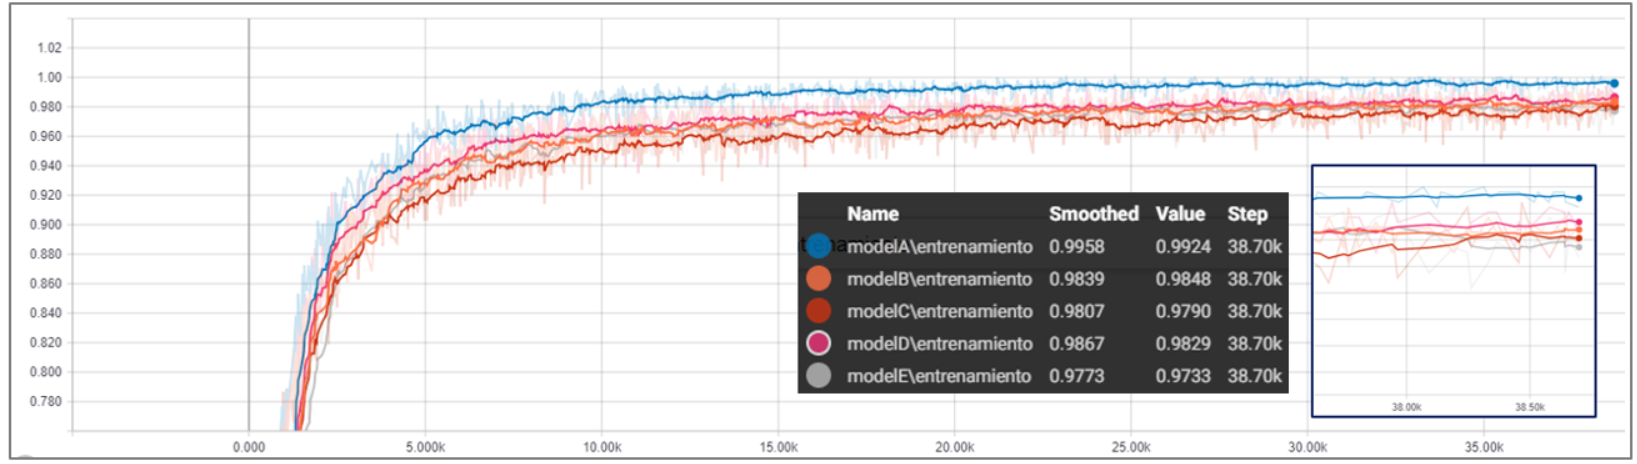
\includegraphics[width=1\textwidth, height=\textheight,keepaspectratio]{images/desarrollo/trainResults/germanSummary_entreAcierto} 
				\caption{\tiny{Análisis del acierto en el Entrenamiento de los modelos - Dataset Señales de Tránsito de Alemania}} 
				%\end{center}
			
	\end{figure}	


}

\frame{
\begin{block}
{\Large{Resultados del Entrenamiento - Dataset Alemania}}
\end{block}
%\vskip 0.5cm
	Los 5 modelos lograron similares resultados de error durante el entrenamiento.
%\vskip 0.3cm


	\begin{figure}[H]
		%\begin{center}
		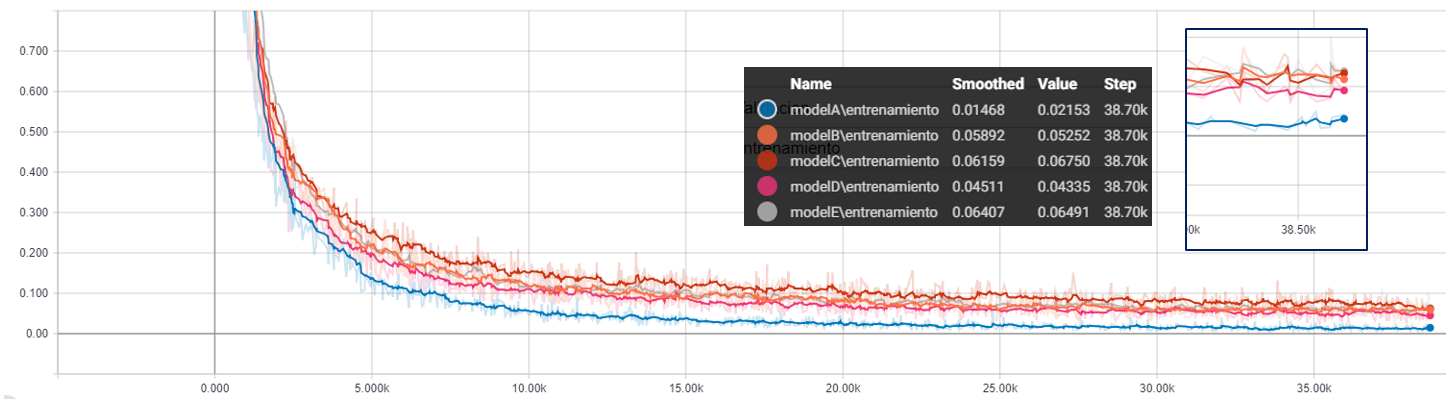
\includegraphics[width=1\textwidth, height=\textheight,keepaspectratio]{images/desarrollo/trainResults/germanSummary_entreError} 
		\caption{\tiny{Análisis del error en el Entrenamiento de los modelos - Dataset Señales de Tránsito de Alemania}} 
		%\end{center}
		
	\end{figure}	
}

\frame{
\begin{block}
{\Large{Resultados de Validación - Dataset Alemania}}
\end{block}
%\vskip 0.5cm
	El Modelo E obtuvo una de las mejores tasas de Acierto. 
%\vskip 0.3cm
	\begin{figure}[H]
		%\begin{center}
		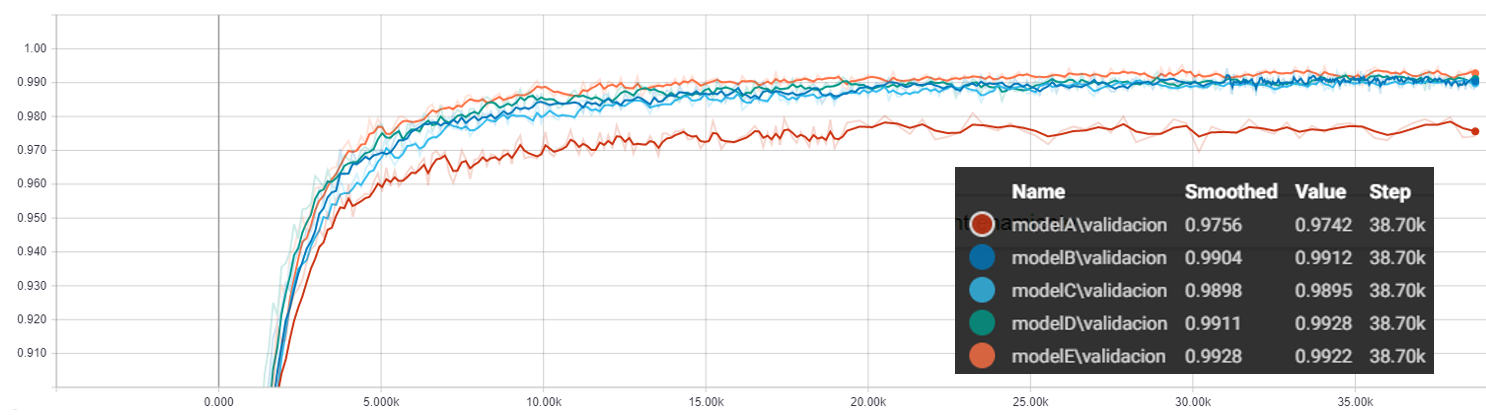
\includegraphics[width=1\textwidth, height=\textheight,keepaspectratio]{images/desarrollo/trainResults/germanSummary_validAcierto} 
		\caption{\tiny{Análisis del acierto en la Validación de los modelos - Dataset Señales de Tránsito de Alemania}} 
		%\end{center}
	
	\end{figure}	

}

\frame{
\begin{block}
{\Large{Resultados de Validación - Dataset Alemania}}
\end{block}
%\vskip 0.5cm
	El Modelo E obtuvo una de las mejores tasas de Acierto. 
%\vskip 0.3cm


	\begin{figure}[H]
		%\begin{center}
		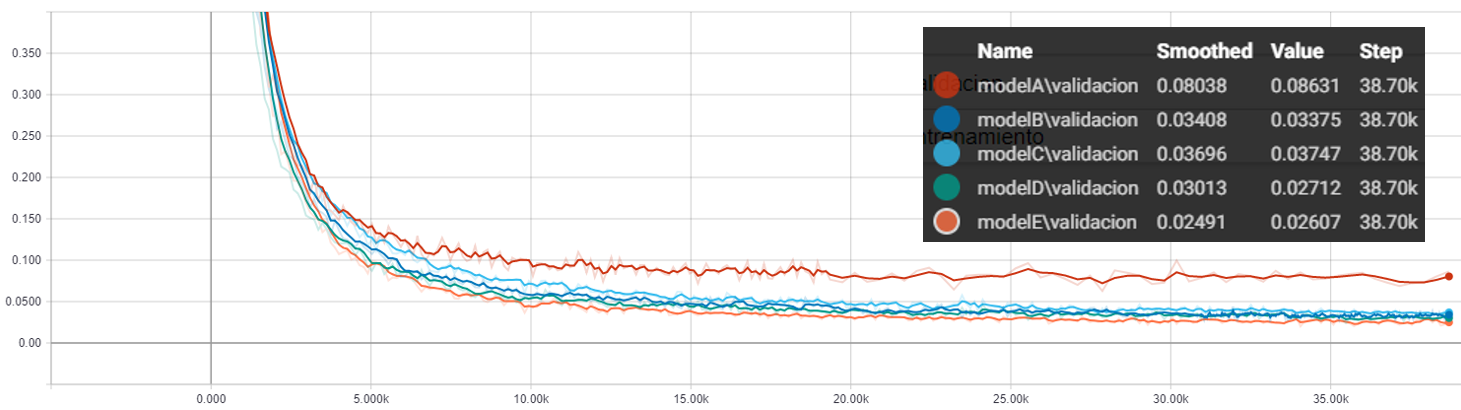
\includegraphics[width=1\textwidth, height=\textheight,keepaspectratio]{images/desarrollo/trainResults/germanSummary_validError} 
		\caption{\tiny{Análisis del error en la Validación de los modelos - Dataset Señales de Tránsito de Alemania}}
		%\end{center}
		
	\end{figure}	
}


%----------------------------------------------------------------------------------------------------------------------
\frame{
\begin{block}
{\Large{Resultados del Entrenamiento - Dataset Perú}}
\end{block}
%\vskip 0.5cm
	Los 5 modelos lograron similares resultados de acierto durante el entrenamiento.
%\vskip 0.3cm
	\begin{figure}[H]
				%\begin{center}
				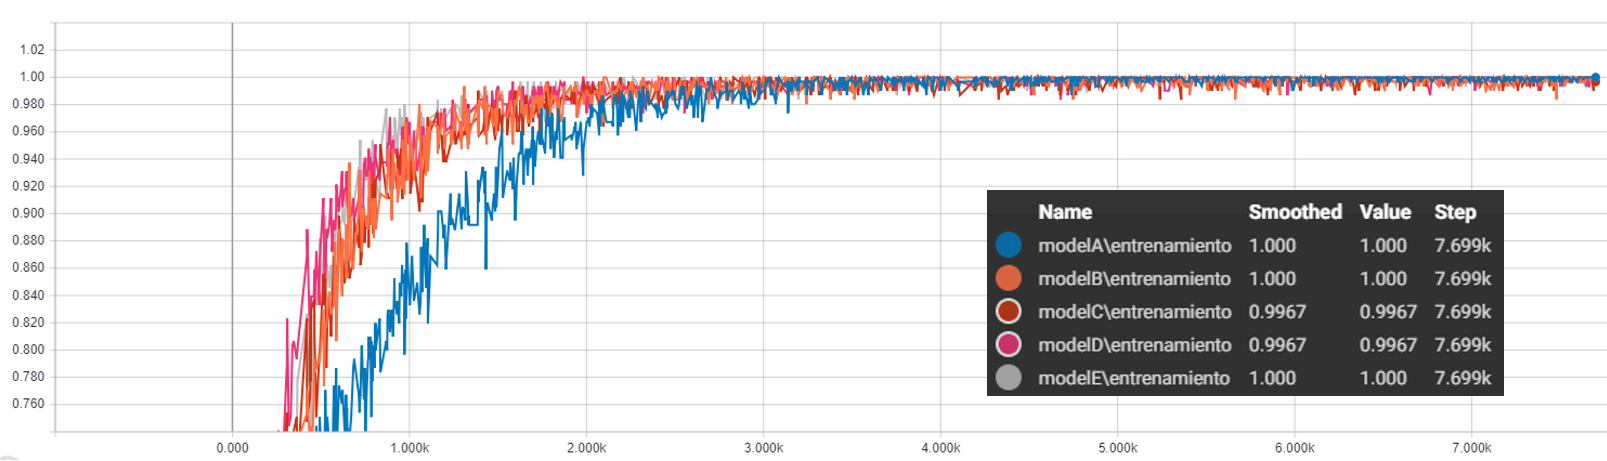
\includegraphics[width=1\textwidth, height=\textheight,keepaspectratio]{images/desarrollo/trainResults/peruSummary_entreAcierto} 
				\caption{\tiny{Análisis del Acierto en el Entrenamiento de los modelos - Dataset Señales de Tránsito de Perú}}
				%\end{center}
			
			\end{figure}	

	
}

\frame{
\begin{block}
{\Large{Resultados del Entrenamiento - Dataset Perú}}
\end{block}
%\vskip 0.5cm
	Los 5 modelos lograron similares resultados de error durante el entrenamiento.
%\vskip 0.3cm


			\begin{figure}[H]
				%\begin{center}
				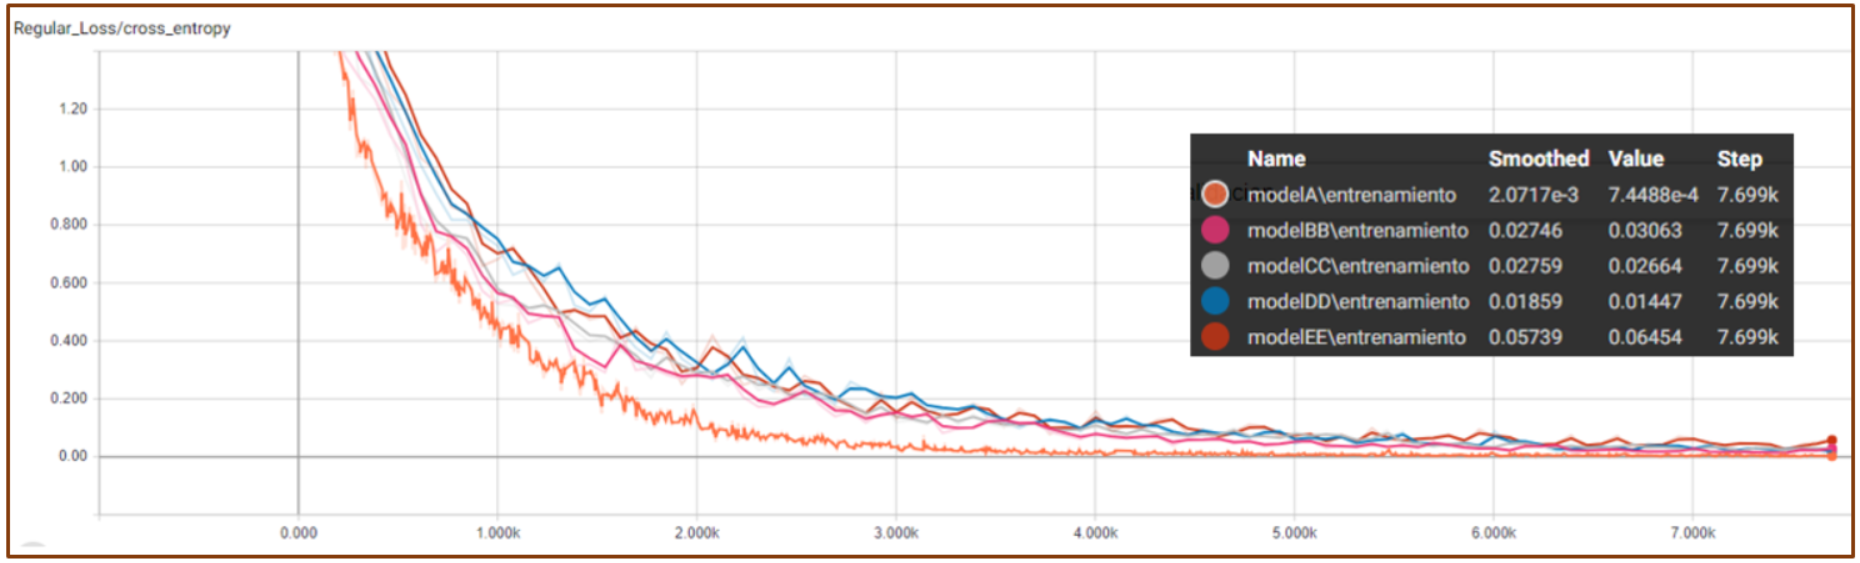
\includegraphics[width=1\textwidth, height=\textheight,keepaspectratio]{images/desarrollo/trainResults/peruSummary_entreError}
				\caption{\tiny{Análisis del Error en el Entrenamiento de los modelos - Dataset Señales de Tránsito de Perú}} 
				%\end{center}
				
			\end{figure}	
}

\frame{
\begin{block}
{\Large{Resultados de Validación - Dataset Perú}}
\end{block}
%\vskip 0.5cm
	El Modelo E obtuvo una de las mejores tasas de Acierto. 
%\vskip 0.3cm
	\begin{figure}[H]
		%\begin{center}
		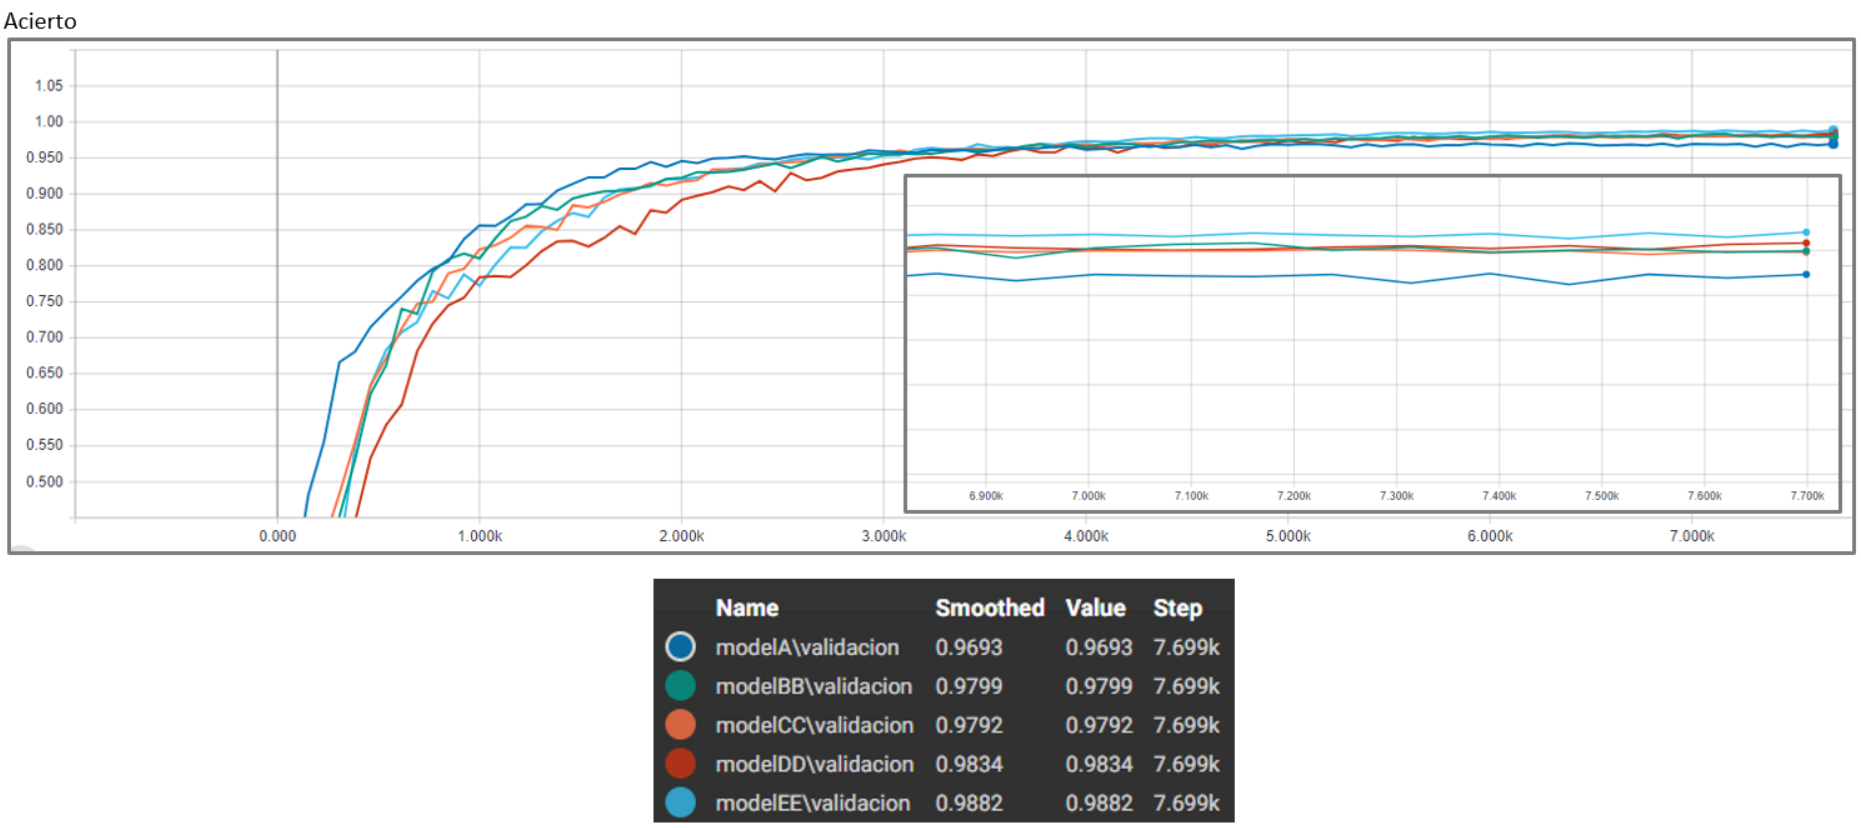
\includegraphics[width=1\textwidth, height=\textheight,keepaspectratio]{images/desarrollo/trainResults/peruSummary_validAcierto} 
		\caption{\tiny{Análisis del acierto en la Validación de los modelos - Dataset Señales de Tránsito de Perú}} 
		%\end{center}
	
	\end{figure}	


}
\frame{
\begin{block}
{\Large{Resultados de Validación - Dataset Perú}}
\end{block}
%\vskip 0.5cm
	El Modelo E obtuvo una de las mejores tasas de Error. 
%\vskip 0.3cm


			\begin{figure}[H]
				%\begin{center}
				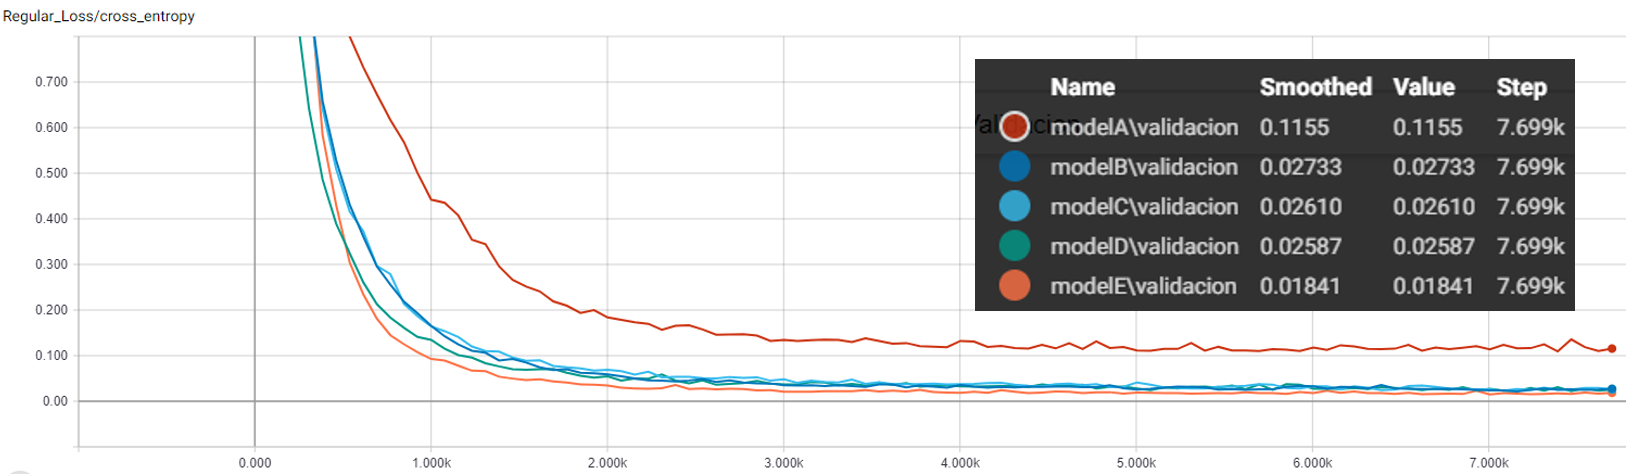
\includegraphics[width=1\textwidth, height=\textheight,keepaspectratio]{images/desarrollo/trainResults/peruSummary_validError} 
				\caption{\tiny{Análisis del error en la Validación de los modelos - Dataset Señales de Tránsito de Perú}} 
				%\end{center}
				
			\end{figure}	
}
